\documentclass[a4paper,12pt]{article}
\usepackage[T1]{fontenc}
\usepackage[toc,page]{appendix}
\usepackage[english]{babel}
\usepackage[utf8]{inputenc}
\usepackage{graphicx}
\usepackage{caption}
\usepackage{subfigure}
\usepackage{indentfirst}
\usepackage{url}
\usepackage[flushleft]{threeparttable}
\graphicspath{{Figures/}}
\usepackage{setspace}
\usepackage[a4paper,left=1cm,right=1cm,top=2cm,bottom=2cm]{geometry}
\usepackage{filecontents}
\usepackage{amsmath}
\usepackage{bbm}
\usepackage{tikz}
\usepackage{float}
\usepackage{setspace}
\usepackage{multirow}
\usepackage{rotating}
\numberwithin{equation}{section}
\DeclareMathOperator*{\argmax}{argmax}
\DeclareMathOperator*{\argmin}{argmin}


\usepackage{geometry}         % Définir les marges
\usepackage{amssymb}

\onehalfspacing

\begin{document}
\setcounter{page}{0} % enlever numéro de page

\begin{titlepage}
    \begin{center}

        \begin{tikzpicture}[remember picture,overlay]
        \node[anchor=north west,yshift=-1.5pt,xshift=1pt]%
        at (current page.north west)
        {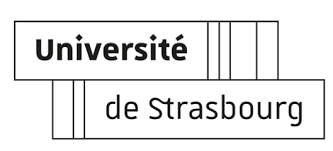
\includegraphics[height=30mm]{LogoUnistra.PNG}};
        \end{tikzpicture}

        \vspace*{4cm}
        
        
        {\Huge\textbf{Comparison of classification algorithms using statistical tests}}
        
        \vspace{0.5cm}
        
        \vspace{1.5cm}
        
        {\LARGE\textbf{Wirtz Kevin}}\\
        \vspace{\baselineskip}
        {\Large University year 2017-2018}
        \vfill
        
        {\Large A Research paper presented for the degree of}\\
        {\Large Statistics and econometrics} 
        
        \vspace{0.8cm}
        
        
\includegraphics[width=0.7\textwidth]{LogoFSEG.png}
        
        
    \end{center}
\end{titlepage} 


\newpage






\tableofcontents
\newpage

\onehalfspacing
\setlength{\parskip}{1em}
\section{Introduction}


In the last few years, machine learning gained a lot of interest, and it stems from two reasons. First, technological progress allows us to perform many tasks in a reasonable time. The fastest supercomputer has a speed of 93 PFLOPS which means $93$ quadrillion operations in one second. This processing power is also available to interested scholars thanks to the use of GPU to perform operations. However, this processing power means nothing if there is no reason to use it. That is where the second reason comes in play: huge amount of data. Google processed 24 petabytes of data per day in 2014 (John Walker, 2014). According to Silver (2013), IBM estimated, in 2012, that 2.5 quintillion bytes of data were produced per day, and at this time 90\% of the data was created during 2010-2012. Because of this, machine learning started to be used in domains like biology, facial recognition, self-driving cars, and others, with results improving state of the art. \par 
The primary goal of machine learning being pattern recognition we can already see the link with Econometrics and Statistics. The border between both of them is thin. Some authors like Charpentier (2015) did some work on the subject.\par 

Cheng et al. (2018) studied the strong relation between neural networks and polynomial regression to try to understand why neural networks give good results while we do not comprehend the reason. The result of this article was the presence of multicollinearity in the different layers of the network. Even though classification problems were not studied, we can see that fundamental questions, as the difference between an old model and the most used algorithm in machine learning, shows interesting results. The goal of this paper is to compare well-known algorithms and popular ones, by using statistical tests. The main question we want to answer is whether popular algorithms used in machine learning give results significantly different from logistic regression. \par

This paper starts with a review of previous studies in Section 2. The next Sections (3,4,5,6) are going to be descriptions of different machine learning algorithms, their intuitions as well as the mathematics behind them. We will then present the experimental setup with the datasets, hyperparameters, and method for statistical testing in Section 7. In Section 8 we discuss the results and in Section 9 we conclude this paper. All python codes and datasets used in this paper can be found on Github: https://github.com/Kwirtz/Masters-thesis.

\newpage

\section{Previous work}

As discussed in Wolpert (2002) no algorithm performs better than every other algorithm for any given problem. The goal of a benchmark is therefore to compare, given a specific set of datasets, different algorithm and give an idea of the strengths and weaknesses of different algorithms to other scholars. A benchmark can also be used to compare general performance which is a major problem in artificial intelligence. The main focus of this paper is to compare the "go-to method" (Cheng et al., 2018), neural network, but also other machine learning algorithms, with logistic regression. \par
Liu et al. (2003) compared different algorithms, such as support vector machines and neural networks, on handwritten digits and concluded that the support vector machine, with a radial basis function as a kernel, performed the best, but they did not perform any statistical test. Lessmann et al. (2015) compared 41 classifier on eight credit scoring datasets using the Friedman test recommended in Demsar (2006). After using the Nemenyi post-hoc procedure to perform a pairwise comparison on four chosen classifiers, they found that neural networks performed better than logistic regression. Garcia et al. (2010) did a benchmark of 48 different datasets. They also used the Friedman test but chose advanced algorithms like evolving radial basis function neural networks or fuzzy support vector learning in their work. Gondara (2016) main focus was the use of different tests on a specific measure of performance and only compared support vector machines and random forests. \par
The goal of this paper would be to follow Lessman et al. but in a more general setting. To the best of my knowledge, there exist no paper on the comparison of multiple classifiers focusing on comparing machine learning algorithms and logistic regression, having a variety of datasets and performing the appropriate statistical tests. Before going into the empirical part of the paper, we will present three machine learning algorithms to grasp the intuition behind them, which is supposed to be known in other benchmark paper and therefore rarely addressed. This theoretical background will allow us to design different classifiers carefully.



\newpage

\section{Support Vector Machine}\label{sec:first}


Support Vector Machine (SVM) is a type of algorithm used in machine learning as a classifier but can also be used in regression problems. The initial groundwork was invented by Vapnik in 1963 but was then improved in 1992 by Boser et al. and 1995 by Cortes and Vapnik. After these two new papers, SVM became popular because it gave better accuracy than the neural network in classification tasks (until deep neural networks which will be discussed later). The primary goal of this section is to go more into the details of the method. To understand SVM, we will first discuss the case where the dataset is linearly separable into two disjoint sets, which will allow for an easier understanding of the logic and also introduce the mathematical notations. Once this is done the generalization in the 1992 and 1995 papers will be straightforward. This section is based on Bishop (2006).


\subsection{Linearly and exactly separable case}

We begin this section of SVM by a two-class classification problem in which we want to separate both classes by a line. Figure 1, based on Hsuan-tien (2018), represents a bulk of point with two dimensions ($x_1$ and $x_2$) and for two distinct populations (red and blue). The first objective is to code an algorithm which identifies these two groups and separate them by a straight line. To make it easier, group 1 is labeled as +1($x_+$ positive example) and group 2 as -1($x_-$ negative example). In each figure, we draw a separating line in a way that the data is perfectly classified. If an observation is above that line, it is classified as group 1, and under that line, it falls in group 2. However, in this example, there is an infinite number of separating lines which respect the condition that every observation is correctly classified. \par
Looking at Figure 1, the last graphic seems, intuitively, to have the best fitting line compared to the two others. A new noisy observation will be close to the data we used to train. Consider the $x_-$ point close to the line of the first panel in Figure 1. A new observation with a slightly higher $X_1$ (The first feature of an observation) will be classified in group one. Therefore points that are, in reality, in group two but differs from the training set because of noise, has a high likelihood to be misclassified (Hsuan-tien, 2018). The first line is said to overfit the data. It classifies our example well but performs poorly confronted with a new observation. 

\begin{figure}[H]%
    \begin{center}
    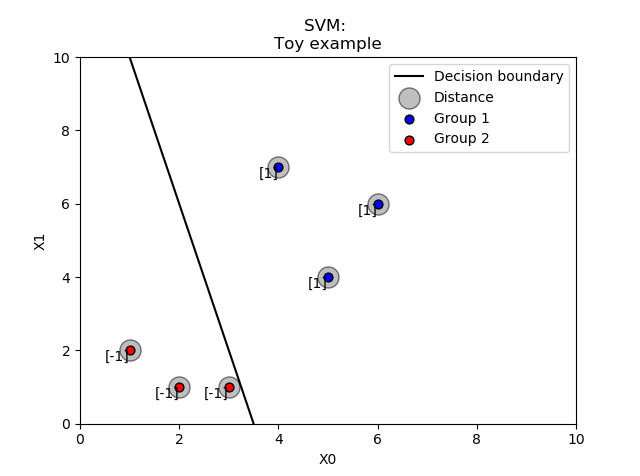
\includegraphics[scale = 0.5]{Figure1SVM.png}%
    \qquad
    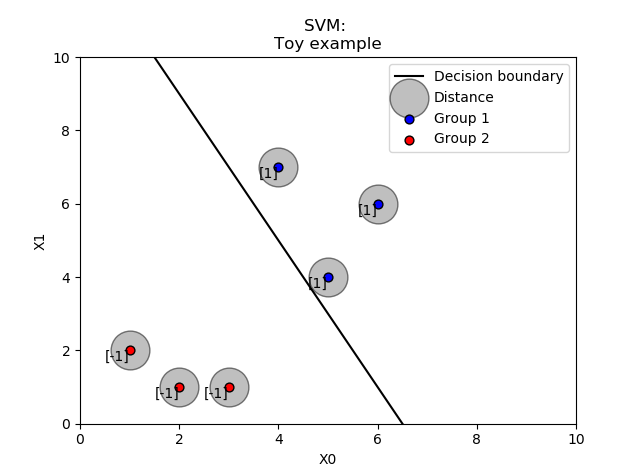
\includegraphics[scale = 0.5]{Figure2SVM.png}%
    \qquad
    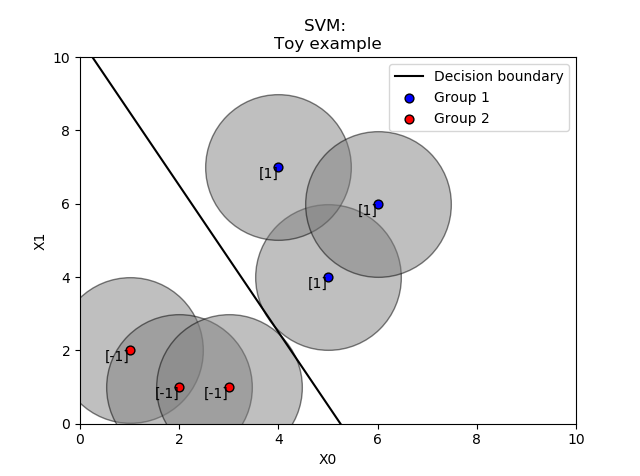
\includegraphics[scale = 0.5]{Figure3SVM.png}%
    \caption{\textbf{Short example of SVM}}%
    \label{fig:example}%
    \end{center}
\end{figure}


Vapnik introduced the concept of margin/gutter (Figure 2). The margin is defined as being the minimum distance between this line, also called hyperplane or decision boundary, and any of the observations. To have the most generalizable line, we find the maximum margin which allows new observations that are close to the training dataset to be still classified correctly. So we want to maximize a minimum, and by doing so, only some points are considered, those who are close to the hyperplane (those who have this minimum distance). The fact that not all the observations are considered is something interesting. The points far away of the decision boundary are not as likely to be falsely classified as the points which are close and therefore the far away observations will not matter in the decision (in Figure 1 the furthest points could have a bigger circle). The fact that the maximum margin solution is the same as minimizing the probability of error is proved by Tong and Koller (2000). So the intuition is: There are two groups, we want to separate them by a line, the SVM procedure gives us a line that satisfies a distance criterion and minimizes the generalization error.

\begin{figure}[H]%
    \begin{center}
    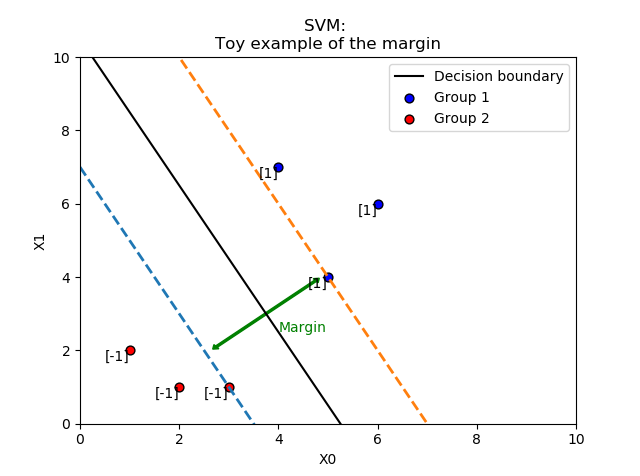
\includegraphics[scale = 0.7]{Figure4SVM.png}%
    \caption{\textbf{Example of the margin}}
    \label{fig2:example}%
    \end{center}
\end{figure}


To represent the process mathematically, we will start by introducing the concept of linear discriminant which is the basis of the support vector machine. The exposition and mathematical notations for this section are taken from Bishop (2006). First, let us define a linear discriminant function:

\begin{equation}\label{eq:1}
f(\boldsymbol{x}) = \boldsymbol{\omega}^T\boldsymbol{x} + b,
\end{equation}

\noindent

where $b$ is a scalar called bias (not in the statistical sense), $\boldsymbol{\omega}$ is called a weight vector and $\boldsymbol{x}$ the input vector. The hyperplane, or decision boundary, is defined by $ f(\boldsymbol{x}) = 0 $. For the moment we will assume that the dataset is linearly separable into two disjoint sets so that there exists at least one pair of parameters $\boldsymbol{\omega}$ and $b$ for which the constraints $f(\boldsymbol{x_+}) > 0 $ and $f(\boldsymbol{x_-}) < 0 $ are satisfied (In other words, all $\boldsymbol{x}$ are correctly classified). Observations $\boldsymbol{x}$ give us information on $\boldsymbol{\omega}$. Consider two observations $\boldsymbol{x}^A$ and $\boldsymbol{x}^B$ which are on this hyperplane. Then $ f(\boldsymbol{x}^A) = f(\boldsymbol{x}^B) = 0 $ hence the result $ \boldsymbol{\omega}^T(\boldsymbol{x}^A-\boldsymbol{x}^B) = 0 $ which means that $\boldsymbol{\omega}$ is orthogonal to the decision boundary.\par
The goals is to find $\boldsymbol{\omega}$ and $b$. The only thing known is that $\boldsymbol{\omega}$ is perpendicular to the hyperplane but there are many orthogonal vectors and orthogonality is not sufficient to identify $\boldsymbol{\omega}$ and $b$. As said earlier there are many lines which separates exactly the dataset in two disjoint subsets. The idea would be to find the solution which overfits the less, or in other words the line which gives us the smallest generalization error. To integrate the concept of margin we start by defining the distance between the decision boundary and any point $\boldsymbol{x}$. As shown in Bishop (2006) this distance is:

\begin{equation}\label{eq:2}
r(\boldsymbol{\omega}, b) = \frac{|f(x)|}{\|\boldsymbol{\omega}\|} = \frac{1}{\|\boldsymbol{\omega}\|}|\boldsymbol{\omega}^T\boldsymbol{x}+b|.
\end{equation}

Equation (3.2) can be rewritten by adding a variable $y_i$ which allows us to get rid of the absolute value.

\begin{equation}\label{eq:3}
    y_i = \begin{cases}
               1               & \mbox{if }\boldsymbol{x_i} \in \mbox{group 1}\\
               -1               & \mbox{if }\boldsymbol{x_i} \in \mbox{group 2} \\
           \end{cases}
\end{equation}

\begin{equation}\label{eq:4}
r(\boldsymbol{\omega}, b) = \frac{1}{\|\boldsymbol{\omega}\|}y_i(\boldsymbol{\omega}^T\boldsymbol{x}+b).
\end{equation}

Now that we have a general formula for the distance, the next step is to write an objective function. We are interested in maximizing the distance between the closest observations. First, we need to find the minimum distance between the decision hyperplane and all the observations in the sample we then search to maximize this minimum with respect to $\boldsymbol{\omega}$ and $b$:

\begin{equation}\label{eq:5}
\max_{\boldsymbol{\omega},b}\{\frac{1}{\|\boldsymbol{\omega}\|}\min_{i}[y_i(\boldsymbol{\omega}^T\boldsymbol{x_i}+b)]\}.
\end{equation} 


However the solution of this program is very complex because of the interdependence between the outer maximization and the inner minimization. We use the fact that the optimization problem is unaffected by rescaling $\boldsymbol{\omega}$ and $b$. Using this property we can set $y_if(\boldsymbol{x_i}) = 1$ for points with the minimum distance. Hence the constraints ($f(\boldsymbol{x_+}) > 0 $ and $f(\boldsymbol{x_-}) < 0 $) become:

\begin{equation}\label{eq:6}
y_i(\boldsymbol{\omega}^T\boldsymbol{x_i}+b) \geq 1, \mbox{ } \mbox{ } \forall i = 1,\dots,N ,
\end{equation}

\noindent
with $N$ being the size of the sample. All points will satisfy (3.6). Among the N observations there exists, at least, two closest points (one for positive and one for negative example) meaning that two or more constraints will be saturated and the minimum in (3.5) becomes, by definition, 1. Therefore the optimization problem only requires to find the solution to:

\begin{equation*}
\max_{\boldsymbol{\omega},b}\frac{1}{\|\boldsymbol{\omega}\|},
\end{equation*}

\noindent
subject to the constraints (3.6). This maximization can be rewritten for mathematical conveniency as:

\begin{equation}\label{eq:7}
\min_{\boldsymbol{\omega},b}\frac{1}{2}\|\boldsymbol{\omega}\|^2,
\end{equation}

\noindent
again subject to the constraints given by equation (3.6). So now we have the object we want to optimize, the constraints (in the form of inequalities), the next logical step is to carry out a Kuhn-Tucker optimization:

\begin{equation}\label{eq:8}
  L(\boldsymbol{\omega},b,\boldsymbol{\alpha})= \frac{1}{2}\|\boldsymbol{\omega}\|^2 - \sum_{i}^{N}\alpha_i[y_i(\boldsymbol{\omega}^T\boldsymbol{x_i}+b)-1],
\end{equation}

\noindent
solving this yields the next equations:

\begin{equation}\label{eq:9}
 \frac{\partial L(\boldsymbol{\omega},b,\boldsymbol{\alpha})}{\partial\boldsymbol{\omega} } = 0 \Longrightarrow \boldsymbol{\omega} - \sum_{i}^{N}\alpha_iy_i\boldsymbol{x_i} = 0 \Longrightarrow \boldsymbol{\omega} =  \sum_{i}^{N}\alpha_iy_i\boldsymbol{x_i}.
\end{equation}

\begin{equation}\label{eq:10}
\frac{\partial L(\boldsymbol{\omega},b,\boldsymbol{\alpha})}{\partial b}  = 0 \Longrightarrow - \sum_{i}^{N}\alpha_iy_i = 0 \Longrightarrow \sum_{i}^{N}\alpha_iy_i = 0.
\end{equation}

The Kuhn-Tucker conditions are:


\begin{align*}
  \alpha_i \geq 0 \\
  y_i(\boldsymbol{\omega}^T\boldsymbol{x_i}+b)-1 \geq 0 \\
  \alpha_i[y_i(\boldsymbol{\omega}^T\boldsymbol{x_i}+b)-1] = 0\\
  \forall i = 1, ..., N
\end{align*}

Putting (3.9) and (3.10) in (3.8) and simplifying gives us the next equation.

\begin{equation}\label{eq:11}
 L(\boldsymbol{\alpha}) = \sum_{i=1}^{N}\alpha_i-\frac{1}{2}\sum_{i}^{N}\sum_{j}^{N}\alpha_i\alpha_jy_iy_j\boldsymbol{x}_i^T\boldsymbol{x}_j.
\end{equation}

Equation (3.11) is the objective function of the dual representation. The Kuhn-Tucker conditions mixed with (3.11) allows us to discuss the former intuition that not all points $\boldsymbol{x}_i$ will matter. If $\boldsymbol{x_i}$ is not on the margins, which means $y_i(\boldsymbol{\omega}^T\boldsymbol{x_i}+b) > 1 $, then $\alpha_i = 0$ and it will not appear in the sum of the dual optimization. Only points for which the constraint is active, and therefore are on the margin, will have $\alpha_i \geq 0 $ and will have an impact on the solution. Once this is done, different optimization algorithms can be performed, such as gradient descent or the most used one in SVM: Sequential Minimal Optimization (SMO) (Platt, 1998). \par
Something to be aware of is that $L(\boldsymbol{\alpha})$ is a function of the dot product of a pair of observations. This result is important because we started that section by having two strong assumptions. One of them was that the dataset is linearly separable. It is not the case for most of the real world data. That is where the paper from Boser et al. (1992) comes into play. 

\newpage
\subsection{Non linearly and exactly separable case}

Vapnik and al. released the linear assumption and created a non-linear classifier by using something called the kernel trick. When we have a non linearly separable dataset we can transform the different inputs $\boldsymbol{x}$ and map them in a higher dimensions, we can denote this transformation: $\phi(\boldsymbol{x})$ with $\phi: R^K \Longrightarrow R^Z$ with $K$ the dimension of the input (in the case of SVM, $K$ is the length of $\boldsymbol{x_i}$) and $Z \geq K$ the dimension of the output which depends on the transformation used. The only thing that changes when we compare it to the basic procedure is that instead of having $\boldsymbol{x}_i$ we have a transformation $\phi(\boldsymbol{x}_i)$. The dot product in the optimization is transformed into $\phi(\boldsymbol{x}_i)^T\phi(\boldsymbol{x}_j)$. But this might become computationally inefficient. For example:

\begin{equation*}
 \boldsymbol{x_i} =
 \begin{bmatrix}
 x_{i1} & x_{i2} 
 \end{bmatrix}^T
\end{equation*}

\begin{equation*}
 \phi(\boldsymbol{x}_i)=
 \begin{bmatrix}
    x_{i1}x_{i1}    & x_{i1}x_{i2} & x_{i2}x_{i1} & x_{i2}x_{i2}\\

 \end{bmatrix}^T; \\
  \mbox{ }
  \phi(\boldsymbol{x}_j)=
 \begin{bmatrix}  
    x_{j1}x_{j1}    & x_{j1}x_{j2} & x_{j2}x_{j1} & x_{j2}x_{j2}\\

 \end{bmatrix}^T
\end{equation*}

\begin{equation*}
\phi(\boldsymbol{x}_i)^T\phi(\boldsymbol{x}_j) = (x_{i1}x_{i1})(x_{j1}x_{j1}) + \dots + (x_{i2}x_{i2})(x_{j2}x_{j2}).
\end{equation*}

Starting with a vector of length two the transformation $\phi$ gives us a vector of length four, then by doing a dot product we will end up with a scalar. We go to a higher dimension (from 2 to 4) and then back to 1 which is computationally inefficient. Also, it is not unusual to go in an even higher dimension. It would be better to go directly from a length of 2 to 1. That is what the kernel trick allows us to do. We do not need to know the transformation of a vector we only need to know the dot product of such transformation. It is not unusual to have the transformation $\phi$ to return a vector with a length that tends toward infinity, that is why the kernel trick is so important.

For this section we are going to make extensive use of the work of Hofmann (2006) which goes in depth into the subject. Let us denote the kernel transformatiosn $k(x_i,x_j)$

\begin{equation*}
 k(\boldsymbol{x}_i,\boldsymbol{x}_j) = \langle \phi(x_i),\phi(x_j) \rangle.
\end{equation*}

The kernel that correspond to the previous example is :

\begin{equation*}
 k(x_i,x_j) = (\boldsymbol{x}^T_i\boldsymbol{x}_j)^2 = (x_{i1}x_{j1} + x_{i2}x_{j2})^2 =  \langle \phi(\boldsymbol{x}_i),\phi(\boldsymbol{x}_j) \rangle.
\end{equation*}



With the kernel trick, the features never go to a higher dimension. The last equations are only a toy example, Cortes and Vapnik (1995) used a transformation with $N(N+3)/2$ coordinates with $N$ the number of observations which can be high as specified in the earlier discussion about the amount of data available. A plethora of kernels exists but here are the most used ones:

\begin{equation*}
\mbox{Linear kernel: } k(\boldsymbol{x}_i,\boldsymbol{x}_j) = \boldsymbol{x}^T_i\boldsymbol{x}_j
\end{equation*}

\begin{equation*}
\mbox{Polynomial kernel: } k(\boldsymbol{x}_i,\boldsymbol{x}_j) = (\boldsymbol{x}^T_i\boldsymbol{x}_j+c)^d
\end{equation*}


\begin{equation*}
\mbox{Radial basis function: } k(\boldsymbol{x}_i,\boldsymbol{x}_j) = exp-(\frac{\|\boldsymbol{x}_i -\boldsymbol{x}_j\|^2}{2\sigma^2}) = exp-(\gamma\|\boldsymbol{x}_i -\boldsymbol{x}_j\|^2).
\end{equation*}


There are different hyperparameters for the kernels (e.g., $c$ for the polynomial and $\gamma$ for the RBF). These hyperparameters can be optimized with a grid-search method (we will discuss this in the empirical setting section). The only thing to make a kernel valid is called the mercer condition. We will not go into the details of what this condition is, but it is something we need to have in mind if we do not make use of the kernels previously presented.

We covered how such a transformation is done but now let us dive into the intuition behind it, and see how it allows us to separate the dataset. By introducing an extra dimension, we will create a measure of similarity. Let us take the radial basis kernel for example. If $\boldsymbol{x}_i$ and $\boldsymbol{x}_j$ are close, we end up with a scalar close to 1 and inversely if they are far away the value will be close to 0. Concerning $\gamma$, since it is the inverse of the variance, a small gamma means a high variance radial basis function which translates to considering points that are far away as similar. The transformation allows for a change of perspective. It is just a change of coordinates to improve the distinction between different points. There might be times where, even though we go into higher dimensions, we will not be able to separate the dataset perfectly, and there will be no solution. As the linearity assumption, we can release the exactly separable assumption.

\newpage
\subsection{Non separable case}

Cortes and Vapnik (1995) wrote another article which allows for flexibility, they called this model the soft margin hyperplane allowing for error in the separation. They do that by adding a slack variable $\varepsilon_i \geq 0 $. If $\boldsymbol{x_i}$ is correctly classified then $\varepsilon_i = 0 $. Points that are correctly classified but are inside the margin have a $\varepsilon_i$ between 0 and 1. Finally, if $\boldsymbol{x_i}$ is misclassified, $\varepsilon_i > 1 $.  The constraint in (3.6) becomes:

\begin{equation}\label{eq:12}
y_i(\boldsymbol{\omega}^T\boldsymbol{x_i}+b)-1+\varepsilon_i\geq 0 \mbox{   } \forall i = 1,\dots,N ,
\end{equation}

And the optimization problem:


\begin{align*}
  \min_{\boldsymbol{\omega},b,\varepsilon} \frac{1}{2}*\|\boldsymbol{\omega}\|^2 + C\sum_{i=1}^{N}\varepsilon_i \\
  \mbox{subject to } y_i(\boldsymbol{\omega}^T\boldsymbol{x}_i+b) \geq 1 -\varepsilon_i\\
  \varepsilon_i \geq 0, \mbox{ } \mbox{ } \forall i = 1,\dots,N.
\end{align*}


$C > 0$ dictates how much an error affects the rest of the equation. Since a misclassified $\boldsymbol{x}_i$ results in $\varepsilon_i > 1$, a high $C$ means that a misclassified observation will have more impact on the objective function, hence to minimize it we allow only a low number of points $\boldsymbol{x}_i$ to be misclassified ( If $ C \rightarrow \infty$ then we want no misclassification, which is the hard-margin case). $C$ is fixed arbitrarily, using cross-validation and grid-search (report to the experimental setup Section). The Kuhn-Tucker optimization problem becomes:


\begin{equation}\label{eq:13}
  L(\boldsymbol{\omega},b,\boldsymbol{\alpha},\boldsymbol{\varepsilon},\boldsymbol{\mu})= \frac{1}{2}*\|\boldsymbol{\omega}\|^2 + C\sum_{j=1}^{N}\varepsilon_j- \sum_{i}^{N}\alpha_i[y_i(\boldsymbol{\omega}^T\boldsymbol{x_i}+b)-1+\varepsilon_i]-\sum_{h=1}^{N}\mu_h\varepsilon_h.
\end{equation}

The two partial derivative of with respect to $ \boldsymbol{\omega} $ and $b$ does not change, but now we have to derivate with respect to $ \varepsilon $

\begin{equation}\label{eq:14}
 \frac{\partial L}{\partial{\varepsilon_i} } = C-\alpha_i - \mu_h.
\end{equation}

In this case, the Kuhn-Tucker conditions are :

\begin{align*}
  \alpha_i \geq 0 \\
  y_i(\boldsymbol{\omega}^T\boldsymbol{x_i}+b)-1 + \varepsilon_i \geq 0 \\
  \alpha_i[y_i(\boldsymbol{\omega}^T\boldsymbol{x_i}+b)-1 + \varepsilon_i] = 0 \\
  \mu_h \geq 0 \\
  \varepsilon_h \geq 0 \\
  \mu_h\varepsilon_h = 0.
\end{align*}


Since $\mu_h \geq 0$ we can deduce from (3.14) that $ \alpha_{max} = C $. The soft margin model is also called C-SVM. Although $\alpha$ is bounded, $C$ is not, and it has no proper interpretation. That is what encouraged Sch{\"o}lkopf et al. (2000) to create another algorithm called $\nu$-SVM. The objective function for it is:


\begin{align*}
  \min_{\boldsymbol{\omega},b,\varepsilon} \frac{1}{2}\|\boldsymbol{\omega}\|^2 - \nu\rho + \frac{1}{N}\sum_{i=1}^{N}\varepsilon_i \\
  \mbox{subject to } y_i(\boldsymbol{\omega}^T\boldsymbol{x}_i+b) \geq \rho -\varepsilon_i\\
  \varepsilon_i \geq 0 \mbox{ } \forall i = 1,\dots,N \\
  \rho \geq 0 \\
  0 \leq \nu  \leq 1.
\end{align*}{}

To understand $\rho$ consider the case where $\varepsilon = 0$, the width of the margin will become $2\rho/(\|\boldsymbol{\omega}\|)$. This result stems from the first constraint wherein the hard-margin SVM we had the arbitrary choice of setting the minimum distance between any point and the hyperplane to one. Once more we can define the Kuhn-Tucker as:

\begin{equation}\label{eq:15} 
 L(\boldsymbol{\omega},b,\boldsymbol{\alpha},\boldsymbol{\varepsilon},\boldsymbol{\mu},\rho,\delta)= \frac{1}{2}\|\boldsymbol{\omega}\|^2 - \nu\rho +\frac{1}{N}\sum_{j=1}^{N}\varepsilon_j- \sum_{i=1}^{N}\alpha_i[y_i(\boldsymbol{\omega}^T{\boldsymbol{x_i}}+b)-\rho+\varepsilon_i]-\sum_{h=1}^{N}\mu_h\varepsilon_h - \sum_{k=1}^{N}\delta_k\rho_k.
\end{equation}

Like for $C$-SVM and SVM the partial derivative with respect to $\boldsymbol{\omega}$ and $b$ are equivalent. But now we add the 2 others:

\begin{align*}
 \frac{\partial L}{\partial{\varepsilon_i} } = -\alpha_i - \mu_i + \frac{1}{N}\\
 \frac{\partial L}{\partial{\rho} } = \sum_{i=1}^{N}\alpha_i - \delta - \nu.  
\end{align*}


By adding the Kuhn-Tucker condition :

\begin{align*}
  \alpha_i \geq 0 \\
  y_i(\boldsymbol{\omega}^T\boldsymbol{x_i}+b)-\rho + \varepsilon_i \geq 0 \\
  \alpha_i[y_i(\boldsymbol{\omega}^T\boldsymbol{x_i}+b)-\rho + \varepsilon_i] = 0 \\
  \mu_h \geq 0 \\
  \varepsilon_h \geq 0 \\
  \mu_h\varepsilon_h = 0 \\
  \delta_k \geq 0 \\
  \rho_k \geq 0 \\
  \delta_k\rho_k = 0.
\end{align*}

We can see that $ 0 \leq \alpha_i \leq \frac{1}{N} $ and $\sum_{i=1}^N\alpha_i \geq \nu $. This $\nu$ is said to be the upper bound of the fraction of margin error (How many points lie on the wrong side of the boundary/for how many points $ \varepsilon_i > 0$). $\nu$ is also the lower bound of the fraction of support vectors (Proportion of points which creates the support vector/ for which $\alpha_i \ge 0$). This interpretation and the convergence between this two boundary (asymptotically: lower bound = upper bound) are prooved in the paper of Sch{\"o}lkopf et al.(2000).

Research has been done ton compare $C$-SVM and $\nu$-SVM and a lot of interesting results emanate from it (Chang and Lin, 2001). There is also the Relevance Vector Machine from Tipping (2001) which allows us to generalize the SVM methodology to a sparse Bayesian approach and therefore add the statistical dimension (for the moment it was only a question of decision boundary) but we lose the convexity property of the optimization problem. \par
We covered all the work that Vapnik and his colleagues did in the 1990's which is still used to this day. 

\newpage
\subsection{Multiclass}

Note that this section is not specific to SVM. Since we are going to use support vector machines in a case of a multiclass problem, we will need to generalize the 2 class approach. For the moment we have only considered the case where we have a positive and negative target value, but in real life application, we often have to partition the observations into more than two groups. Two methods can be used to solve this problem (Bishop, 2006): The single optimization approach and the binary approach (which is in turn decomposed in different algorithms). The single optimization problem tries to solve directly and for all of the class simultaneously. The binary approach is a combination of different optimizations problems and then, using a voting approach (how many of them did put this new observation in this category), we predict the class. The binary solution is usually the one used. We will concentrate our effort on this one. \par
The binary approach is usually divided into two categories: the one-versus-all(OVA) and the one-versus-one (OVO). The OVA approach consists in considering all the points and test one class against all of the others. One major complication of this solution is that the positive examples will be a small fraction of the whole. If we have five classes of equal lengths, then the positive sample will represent 20\% and will be put against the other 80\% which facilitates the misclassification of the positive example. Rifkin (2004) showed the utility of the OVA approach. On the other hand, OVO approach consists only in considering the groups by pairs and do the classification between all of the pairs existing which is less computationally efficient than OVA, and it might lead to ambiguities (Bishop, 2006). Much literature exists on this subject. We are only going to use rudimentary approaches in our benchmark. Therefore we will not go deeper into the theoretical background. Interested scholars can find an extensive list of different approaches from different authors in Rifkin (2004) . This concludes the first section concerning SVM.



\newpage

\section{Tree-based models}\label{sec:second}

The second algorithm we shall use in the benchmarking is Random Forest (RF). First introduced by Breiman (2001), a random forest is a combination of decision trees (CART, ID3, ...) and the concept of bootstrap aggregating (bagging) also presented by Breiman (1996). We will start the discussion by reviewing the base algorithm of decision trees, the construction, the limits and why an ensemble learning method is necessary. We then discuss the bagging method and finish by combining both to introduce random forests. The mathematical notations and intuitions are based on Hastie et al. (2008) in addition to the two articles already mentioned.

\subsection{Decision tree}

A decision tree is a sequential decision algorithm in which the input space is partitioned into a set of rectangle region. This type of method can be used for classification as well as regression. The goal is to predict a class or value $Y$ based on the feature space $X = (X_1,X_2,...,X_p)$. We focus on binary trees where each node splits into two other nodes which makes the understanding more intuitive. At each node, we test a feature which then results in a split in the tree. In other words, at each step, we split a region into two subregions. The choice of features, as well as the split-point, will be discussed later. \par
Let us take an example, starting at the top of the tree we first choose the feature $X_1$ and split it at a point $t_1$ called the threshold. We obtain two subregion $X_1 \leq t_1$ and $X_1 \ge t_1$. For each subspace we, once more, choose a feature and a split point and repeat the operation. Figure 3, from Hastie et al. (2008), shows such a process. For a new point $X$ we start at the top of the tree, also called root node, and follow the path depending on the different values of the features, to end at the last node, also called leaf. The value of y is then defined at the last node and depends on the type of problem. 

\begin{figure}[H]%
    \begin{center}
    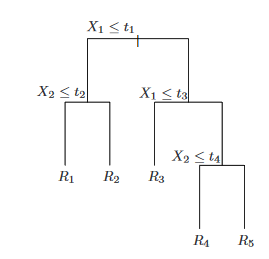
\includegraphics[scale = 0.8]{Figure1RF.png}%
    \qquad
    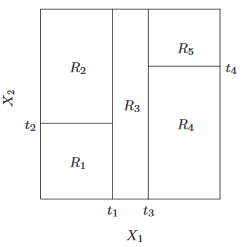
\includegraphics[scale = 0.8]{Figure2RF.png}%
    \caption{\textbf{Example of decision tree (Hastie et al. 2008)}}%
    \label{fig:DecisionTree}%
    \end{center}
\end{figure}


We described the basic procedure of a decision tree, but we still need to decide a way to choose the feature to split and the threshold of the splitting. There are numerous algorithms the main ones being CART (classification and regression trees) and C4.5 but we can also mention CHAID or MARS. Our primary focus will be the CART. 

We shall first discuss the case of a regression problem. We have $N$ observations, each with $p$ features and a response value. The data is composed by the features $\boldsymbol{x}_i=(x_{i1},\dots,x_{ip})$ and the response value $y_i$ which is a continuous variable in the regression case. If the tree is already fixed, meaning we partitioned the space in M regions $R_1,...R_M$, we attribute a constant $c_m$ for each region such that a new observation $\boldsymbol{x}$ who falls in space $R_m$ will have a response value of $c_m$. In other words the prediction, $c_m$ of a new observation will depend on the space $R_m$ it falls in. This allow us to write the prediction made for $\boldsymbol{x}$ in the form:

\begin{equation}\label{eq:1}
f(\boldsymbol{x}) = \sum_{m=1}^Mc_m \mathbbm{1}(\boldsymbol{x} \in R_m).
\end{equation} 

The error function, when using the sum of squared error, is then defined by :

\begin{equation}\label{eq:2}
\sum_{i=1}^N (y_i - f(\boldsymbol{x}_i))^2.
\end{equation} 

Minimizing this error function with respect to $c_m$ for $m = 1,\dots,N$ the solution is:

\begin{equation}\label{eq:4}
\hat{c}_m= \frac{1}{N_m}\sum_{i \in R_m}y_i, 
\end{equation} 

\noindent
where $N_m$ is the number of observation in $R_m$. This result shows that the prediction that minimizes the error is a local average of the response variable.The last step is to find the fixed tree that we used to predict (in other words we need to create the different $R_m$). We still need to define the number of splits, which features to choose and the threshold to split. We could use the same concept as we did before and use the sum of squared error function but due to the number of combination between all the elements, it is computationally infeasible. To solve the problem, we will perform a heuristic algorithm. These algorithms are also called greedy algorithms and describe a recursive process in which we perform a locally optimal choice at each step, in the case of decision tree at each node, and do this multiple time until an optimal solution is found. To perform such a procedure let us start at the top of the tree, at this point there exist a unique region and all the observation is included in this space. We consider the variable $j$ to split and the threshold to be $t$. Once we split the starting space, two regions emerge and are defined by:

\begin{equation}\label{eq:5}
R_{1}(j,t) = \{\boldsymbol{X}|x_j \leq t\} \mbox{ and }R_2(j,t) = \{\boldsymbol{X}|x_j>t\},
\end{equation} 

where $\boldsymbol{X}$ is the matrix of all the observations and covariates, hence the dimension of such matrix is $N$x$p$. Once more we use the sum of squared error function to minimize the error of prediction for each region but we also want that the sum of the error of the two regions are the smallest with respect to the feature selected and the split point. Hence the optimization problem is :

\begin{equation}\label{eq:6}
\min_{j,t}[\min_{c_1}\sum_{\boldsymbol{x}_i \in R_1(j,t)}(y_i-c_1)^2 + \min_{c_2}\sum_{\boldsymbol{x}_i \in R_2(j,t)}(y_i-c_2)^2].
\end{equation} 


Note that earlier we explicitly wrote that $c_m$ depends on $R_m$, now we also see that the choice of $R_m$ depends on the error function which, itself, contains $c_m$. As seen previously, both minimization with respect to $c_1$ and $c_2$ are a local average in the respective region. To solve the outer minimization, we find the optimal $t$ for each variable. This is considered as a fast process hence we can perform an exhaustive search. The next step is to select the variable with the splitting point which gives the smallest error. This process of splitting can go as long as we want. A deeper tree will have a better accuracy until we have perfect accuracy, in other words, the tree will overfit.\par
To solve this problem the straightforward intuition would be to stop when the gain of a new separation for the error function is low, but Hastie et al.(p.308) mention that after multiple splits where the error function is almost constant, a new one can suddenly improve the accuracy of the model. Hence we need another way to help us decide the number of splits in a tree. The CART methodology solves this problem by growing a large tree $T_0$, which contains an arbitrary number of splits, and then pruning the tree to find a subtree $T$. This pruning consists of collapsing internal nodes and replacing it with a leaf node which is just the average of the later leaves node. Let us start by defining the evaluation of the error for a given tree, T, with the three following equations:

\begin{align*}
N_m = \sum_{i=1}^N \mathbbm{1}(\boldsymbol{x}_i \in R_m) \\
\hat{c}_m = \frac{1}{N_m}\sum_{\boldsymbol{x}_i \in R_m}y_i \\
Q_m(T) = \frac{1}{N_m}\sum_{\boldsymbol{x}_i \in R_m}(y_i-c_m)^2.
\end{align*} 

$Q_m(T)$ is the contribution to the error function of the region m. Let us define $|T|$ as the number of final nodes in T. The pruning criterion is then given by:

\begin{equation}\label{eq:7}
C_{\alpha}(T) = \sum_{m=1}^{|T|}N_mQ_m(T)+\alpha|T|.
\end{equation}

The complexity of the model is measured by $|T|$ and governed by $\alpha$. The idea of complexity pruning is to find the subtree in such a way to minimize $C_{\alpha}(T)$. Hence $\alpha$ manages the tradeoff between complexity and goodness of fit. If $\alpha = 0$ then the optimal subtree is $T_0$ in the case where $\alpha = +\infty$ then the optimal subtree, called null tree, is a single leaf node, the root node. To find the optimal subtree, we use a method called weakest link pruning. We start with the tree $T_0$ we then replace a subtree by a leaf node and obtain a new tree $T_1$. We build every tree possible from $T_0$ and choose which of them, and therefore which nodes, produce the smallest decrease in the error. We repeat this operation until we reach the root node. This procedure will give us values for $\alpha$ and an optimal tree associated with it. The last step is to choose $\alpha$ and the recommended way is using cross-validation.

In the case of a classification problem the procedure stays the same but the prediction of the response variable then becomes a majority vote instead of an average. In other words the class the most frequent in this region is predicted. Let us define $\hat{p}_{mk}$ the proportion of observation that are class k in region m:


\begin{equation}\label{eq:8}
\hat{p}_{mk} = \frac{1}{N_m}\sum_{\boldsymbol{x}_i \in R_m} \mathbbm{1}(y_i = k).
\end{equation}

The prediction k(m) is then the highest proportion. The last thing to change is the way to choose the feature and the split point and, as for the prediction, the only thing to change is the measure of error which was the squared error function for regression. For classification there exist different measures:

\begin{align*}
\mbox{Missclassification error: } \frac{1}{N_m}\sum_{x_i \in R_m}\mathbbm{1}(y_i \neq k(m)) = 1- \hat{p}_{mk(m)} \\
\mbox{Gini index: }\sum_{k=1}^K \hat{p}_{mk}(1-\hat{p}_{mk}) \\
\mbox{Cross-entropy: } - \sum_{k=1}^K \hat{p}_{mk} log\hat{p}_{mk}.
\end{align*} 

In the regression case, we used the same error function for the construction of the tree but also for the pruning algorithm. In general, in a classification problem, The Gini index and cross-entropy are used for the growing part because of their derivative properties while for pruning misclassification rate is used for simplicity. 

One of the main advantages of a tree model such as CART is the interpretability of the results. They also perform a feature selection implicitly and are faster to train than algorithms like neural networks. Conversely, the main problem with decision trees is their sensitivity to the dataset. In other words, the variance of the tree is high which it prevents the robustness of the model. According to Hastie et al. this variability is because the tree evolves from the first node. The error is therefore propagated down and is dependent on the initial conditions. A slight change to the first split can result in a significant variation of the prediction. The trade-off bias-variance is not the only problem but one of the most important since it results in overfitting. We focus on a way to reduce this variance, and the solution is bootstrap aggregating (bagging).

\newpage
\subsection{Bagging}

The idea is to use a bootstrap methodology to improve the out-of-sample accuracy of the prediction by reducing the variance of the decision tree. Bootstrap is a resampling technique in which we randomly draw, with replacement, a new dataset from the original dataset and then fit the model on each dataset. In doing so, we can examine different aspects of the distribution of an estimate like the mean or the variance. In the case of bagging, the object we want to evaluate is the prediction of a class or value. In other words, we build $B$ samples, for each sample we create a tree. To predict a new value $y$, we start with input $\boldsymbol{x}$ and pass it through each tree. In a regression case, the predicted value of $y$ from all the trees are averaged, which give us the new, more stable, prediction. When $y$ is a discrete value (class) the new prediction is the mode of all the predictions, this procedure is also called "voting" meaning each tree "vote" in which category we should classify $\boldsymbol{x}$, and the majority wins. 

Let us define the dataset as $Z = \{(\boldsymbol{x}_1,y_1),(\boldsymbol{x}_2,y_2),\dots,(\boldsymbol{x}_N,y_N)\}$ the dataset, with $N$ being the total number of observations in the training set. $Z$ is then resampled using bootstrap so that we have B different sample denoted $Z^b$ where $b = 1,\dots,B$. We then perform the decision tree algorithm seen in the last subsection without pruning since pruning is a way to avoid overfitting which is already done thanks to the bootstrap methodology. For a new input $x$ we then define $\hat{f}^b(x)$ as the prediction given by the model trained on sample $Z^b$. Hence the bagging prediction is:

\begin{equation}\label{eq:9}
\hat{f}_{bag}(\boldsymbol{x})= \frac{1}{B}\sum_{b=1}^B\hat{f}^b(\boldsymbol{x}).
\end{equation}

Breiman (1996) also introduced out-of-bag (OOB) estimation. To check for overfitting, a train/test methodology is often used in machine learning in which we split the dataset in two, use one part for training and then estimate out of sample error with the testing set. The idea behind OOB resembles this method. Breiman used the fact that in bagging we first create $B$ datasets with resampling, this results in having some of the observation not appearing in some trees. In the original paper, Breiman evaluated the proportion of observations that are not present in a fixed tree and gave a rough estimate of 37\%. Knowing this, he created an out-of-bag error which consists in predicting an observation with trees which are not constructed using said observation. Doing this for every point gives us an estimate of generalization error. By comparing the OOB error between different models with different hyperparameters, it can give us an idea of which are the most overfitting without holding out samples (which can be a problem for a small dataset).

Bagging is called an ensemble learning method since its procedure is to aggregate different model. Bagging can be applied to other models than decision trees but only works well for high variance models, in other words, overfitting models (Breiman, 1996). Assuming the trees are i.i.d and $\sigma^2$ is their variance then $(1/B)\sigma^2$ is the new variance which shows that, as $B$ (the number of trees) increase, the variance is decreasing hence the ensemble learning method is justified. However the independently distributed, in other words, there is no correlation between each tree, is a strong assumption. In cases where the trees are only identically distributed (which is true when using bootstrap) and not independently, Hastie and al. (2001) showed that the variance of the trees becomes:

\begin{equation}\label{eq:10}
\rho\sigma^2 + \frac{(1-\rho)}{B}\sigma^2,
\end{equation}

\noindent
with $\rho$ the correlation between pairs of trees. As in the i.i.d case the variance is reduced as $B$ increases, but, in this case, the left element remains unchanged. This lower bound variance motivated further research as bagging had this limit and performed poorly compared to other boosting like AdaBoost. Breiman (2001) proposed, following different papers with the same idea, to add more randomness to the procedure and created the random forest. 


\subsection{Random forest}

The idea of random forest is building on the bagging model. The difference is that each tree, instead of having $p$ input variable, we randomly select a subset of $m$ covariates with $ p\geq m$. A good rule of thumb for m could be  $\sqrt{p}$ as proposed by Hastie et al. (2008). Breiman (2001) used $m = (log_2p+1)$. By doing this randomization, we will reduce, to a certain degree, the dependence of each tree by not working on the same set of variable. Hence $\rho$ in (3.10) becomes smaller as does the variance of the average.\par
Bagging is often compared to another ensemble learning method called boosting. In most cases, it was shown that boosting performed better in term of accuracy for the testing sample (observation not used for training) than bagging. By going a step further and using the random forest, we could approach boosting result with a much faster algorithm. The last thing to note about the random forest algorithm is that it does not require pruning since the biais-variance tradeoff is managed by the number of trees in the forest.

This closes the section about tree-based models. The next algorithm is the most popular one today, deep neural network.


\newpage

\section{Deep Neural Network}\label{sec:third}


The recent interest in machine learning stems from the deep learning branch in which the deep neural network is the core concept. We already talked about how most of the real world underlying processes are nonlinear and deep neural networks (DNN) are suitable to model nonlinearities. The deep neural network has its origin in the perceptron algorithm which is a linear discriminant model created by Rosenblatt (1962) in an attempt to represent information processing in the brain. Another name for the deep neural network is "multilayer perceptron" even though Bishop (2006) warns us about the fundamental difference between both algorithms. \par
This section is structured as follows. First, we will see the basic architecture of the perceptron and generalize it to obtain the deep neural network. Then we will discuss the backpropagation algorithm which is how the parameters of the network are optimized. Finally, we will learn how to avoid overfitting and have a discussion about the hyperparameters in the model. For this section we will make extensive use of Bishop (2006) but also Lecun et al. (1998).

\subsection{Deep Neural Network architecture}

We shall start by presenting the perceptron algorithm. Since it is a two-class linear discriminant model we can use the same linear discriminant function as in SVM. Following Bishop's notation (3.1) becomes:

\begin{equation}\label{eq:1}
y(\boldsymbol{x}) = f(\boldsymbol{\omega}^T\phi(\boldsymbol{x})),
\end{equation}

\noindent
with $\boldsymbol{x}$ the input vector, $\phi$ a nonlinear transformation applied to $\boldsymbol{x}$ which results in the feature vector $\phi(\boldsymbol{x})$ and $\boldsymbol{\omega}$ the weights vector. Note that compared to the form we used in (2.1) the bias term is included in $\phi(\boldsymbol{x})$ such that $\phi_0(\boldsymbol{x})=1$. $f$ is a nonlinear function, called activation function, of the form:

\begin{equation}\label{eq:2}
    f(a) = \begin{cases}
               +1               & \mbox{if }a \geq 0\\
               -1               & \mbox{if }a <0, \\
           \end{cases}
\end{equation}

Usually, in machine learning application, the true output value, named $t$, is encoded with binaries which means that for a two-class problem we should have:

\begin{equation}\label{eq:3}
    t_i = \begin{cases}
               1             & \mbox{if }i \in C_1\\
               0              & \mbox{if }i \in  C_2, \\
           \end{cases}
\end{equation}

\noindent
with $C_1$ for class 1 and $C_2$ for class 2. Here, since the activation function maps the output to either 1 or -1, we will use a target value of $t_i = 1$ if the sample point is in group 1 and $t_i = -1$ if it falls in group 2. 

Finding optimal values of $\boldsymbol{\omega}$ could be seen as complex since the activation function is discontinuous and constant. To realize the difficulty, Bishop proposed to consider the case where the total number of misclassified patterns are chosen as an error function. The usual way to optimize it would be to use the gradient of this error function with respect to $\boldsymbol{\omega}$, but since this error function is constant everywhere, the gradient will be 0 which makes it impossible to update the weights. That is why Rosenblatt considered an error function called the perceptron criterion:

\begin{equation}\label{eq:4}
E_p(\boldsymbol{\omega}) = - \sum_{i \in M}\boldsymbol{\omega}^T\phi(\boldsymbol{x_i})t_i,
\end{equation}

\noindent
where $M$ is the subset of misclassified observations. In other words, when the observation is correctly classified then it is not taken into account in the error function, $E_p(\boldsymbol{\omega}) = 0 \mbox{ }\forall i \notin M$. Once we have defined the error function, we can perform the gradient descent algorithm and find the optimal $\boldsymbol{\omega}$. We will not go into more details on the perceptron algorithm. All the key elements necessary to the understanding of neural networks have been given. In summary, the perceptron consists in having an input $\boldsymbol{x_i}$, multiply it by weights, and then the result is passed through an activation function giving us an output.

The only difference between the architecture of the perceptron and the deep neural network is that the process (input -> activation -> output) will be repeated multiple times and we will not be using the step function as an activation function. To illustrate let us discuss the case of a two-layer network step by step.

Starting once more with equation (\ref{eq:1}), but rewritten as:

\begin{align*}
  a_j = \sum_{i=1}^{D}\omega_{ji}^{(1)}x_i + \omega_{j0}^{(1)} \\
  z_j = h(a_j). \\
\end{align*}

Let us start with the first equation. $D$ is the dimension of the input variable $\boldsymbol{x} = (x_1,\dots,x_D)$. $j = 1,\dots,M$ with M being an arbitrary number of output. M will be discussed in the hyperparameters subsection. $\omega_{ji}^{(1)}$ is the weight associated to input $i$ and the output $j$, and the superscript indicating the current layer. $\omega_{j0}^{(1)}$ is the bias associated with output j in the first layer. The scalar $a_j$ is named activation. Once all the $a_j$ are calculated we pass them through an activation function which is not a piece-wise constant function as in the perceptron but a differentiable, nonlinear activation function $h(.)$ which gives us the second equation. At this point, the process is the same as the perceptron but now instead of having the final output which answers the question of the two-class problem we have M outputs. We still need to go from dimension $M$ to dimension $K$ (with $K$ the number of classes). To do that we will reproduce the same step, but instead of using $x_i$ as the input we will use $z_j$:


\begin{align*}
  a_k = \sum_{j=1}^{M}\omega_{kj}^{(2)}z_j + \omega_{k0}^{(2)} \\
  y_k = \sigma(a_k), \\
\end{align*}

\noindent
this time $M$ is the dimension of the input $\boldsymbol{z} = (z_1,\dots,z_M)$. $k = 1,\dots,K$ with $K$ being the total number of classes. $\omega_{kj}^{(2)}$ is the weight associated to input j and the output k in the second layer and $\omega_{k0}^{(2)}$ is the bias associated to output k in the second layer. Since we use the last layer outputs to calculate the output of a new layer the process is called forward propagation. The choice of the activation function, $\sigma(.)$, will depend on the problem we are facing. In the case of a binary classification problem, a sigmoid function is used:

\begin{equation}\label{eq:5}
\sigma(a) = \frac{1}{1+exp(-a)}.
\end{equation}

In the case of a multiclass problem, we use the softmax function:

\begin{equation}\label{eq:6}
\sigma(a_k) = \frac{exp(a_k)}{\sum_{j=1}^{K}exp(a_j)}.
\end{equation}

If we combine the first layer and the second layer in a single equation we obtain:

\begin{equation}\label{eq:7}
y_k(\boldsymbol{x},\boldsymbol{\omega}) = \sigma ( \sum_{j=1}^{M} \omega_{kj}^{(2)} h(\sum_{i=1}^{D}\omega_{ji}^{(1)} x_i + \omega_{j0}^{(1)} ) + \omega_{k0}^{(2)}).
\end{equation}

We could also include the bias in the weights as in the perceptron, resulting in a more explicit equation. The previous example is only a two-layer network, but other layers could be added by following the same step multiple times (as long as the activation function in the last layer is a logistic or a softmax function for classification problems). Since we used the mathematical notation of Bishop, we also used his neural network representation for coherence. Figure 3 shows an example of the neural network architecture and illustrates the forward propagation process.

\begin{figure}[htb]%
    \begin{center}
    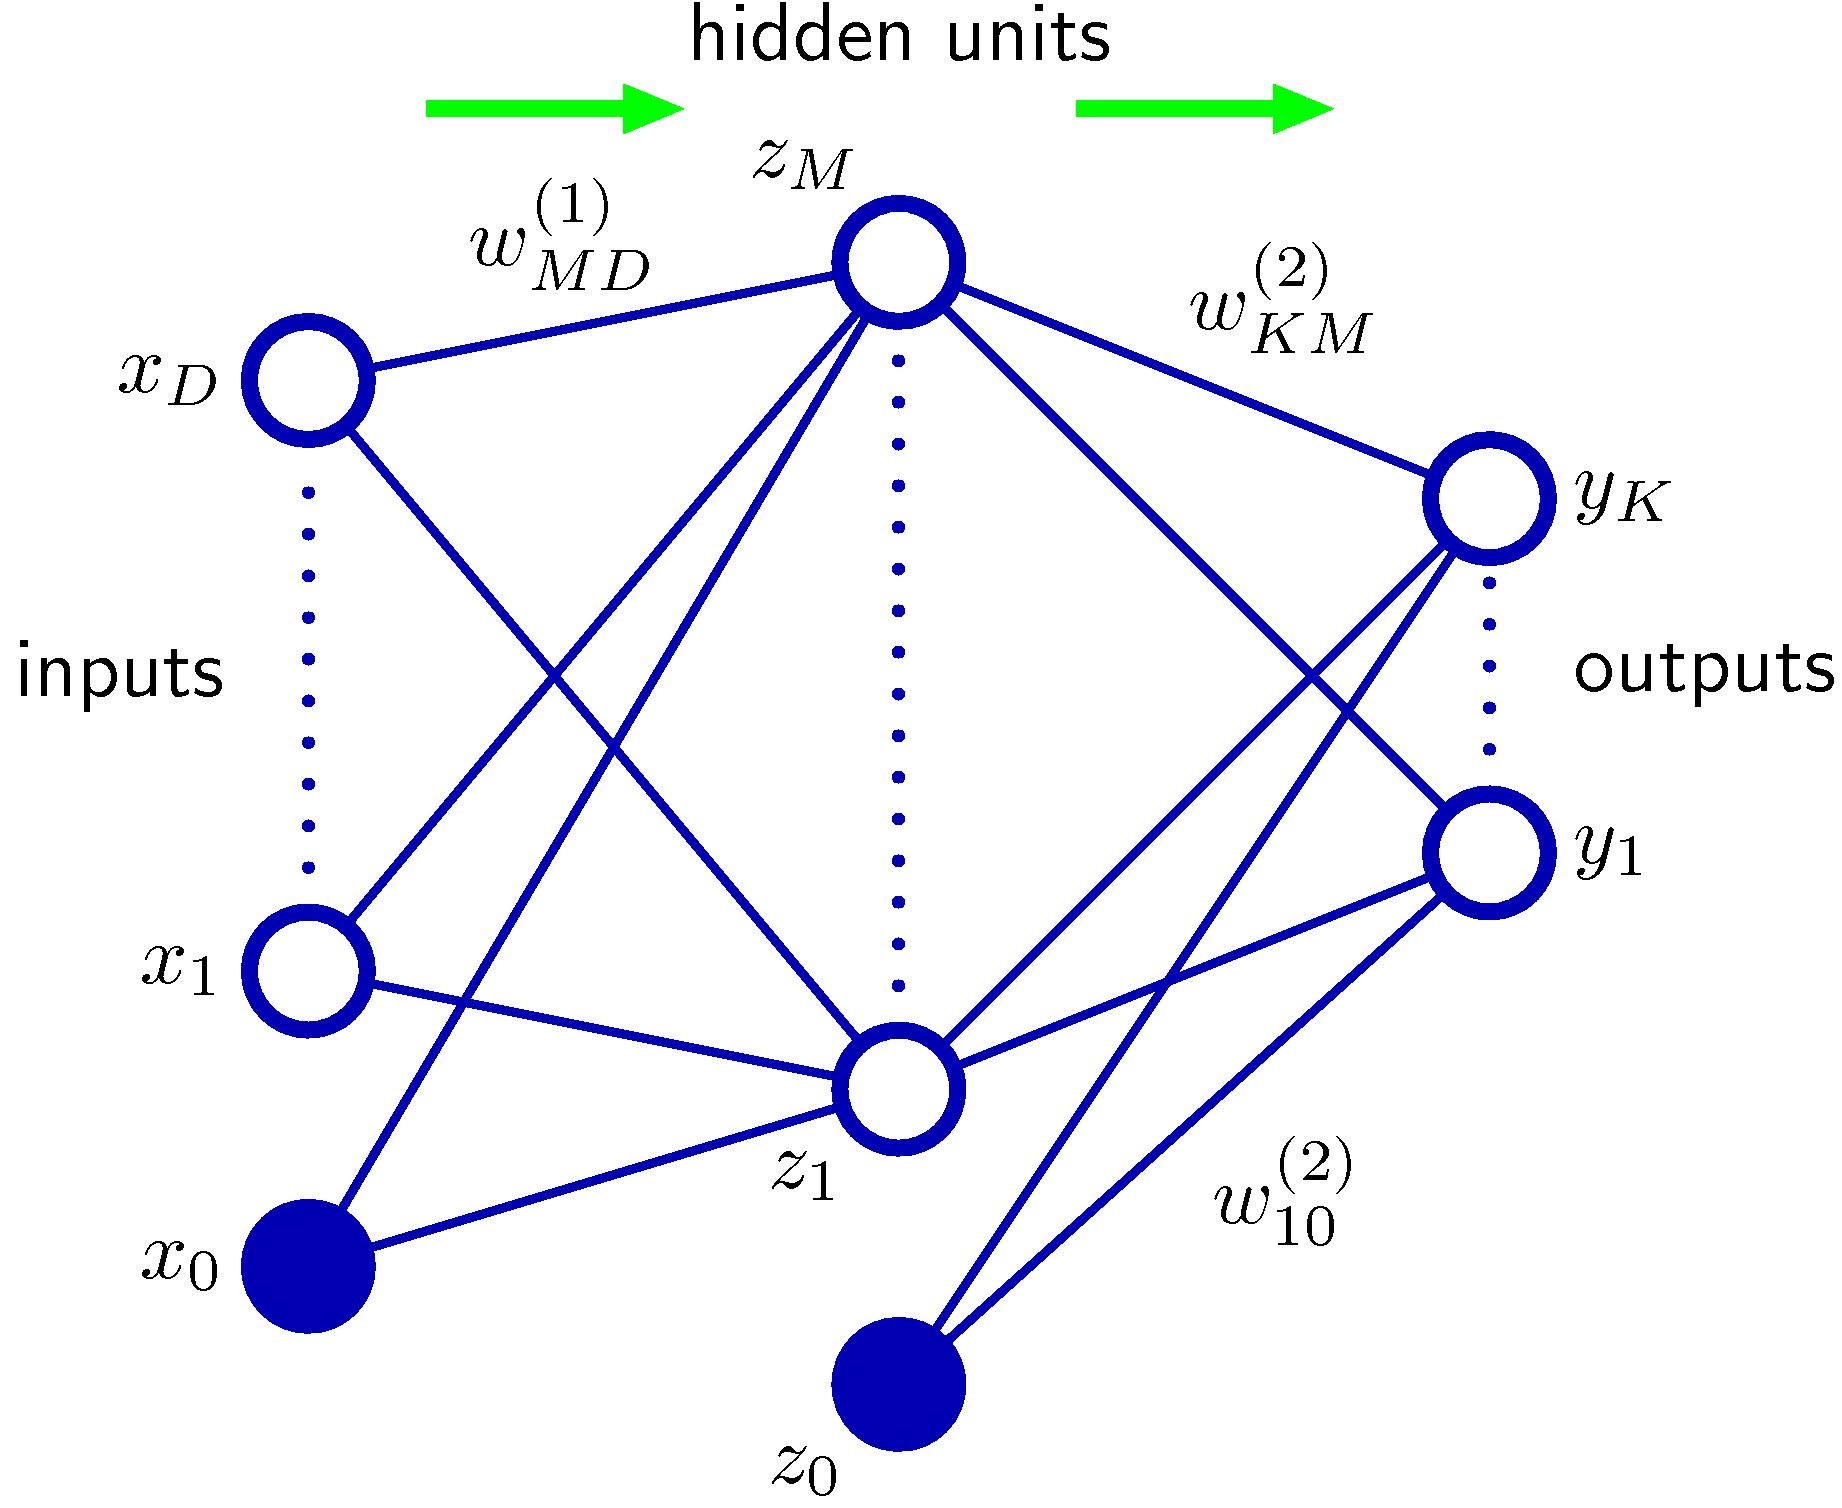
\includegraphics[scale = 1]{Figure1ANN.png}%
    \caption{\textbf{Example of a neural network architecture in a case of $K$ groups (Bishop 2008)}}
    \label{fig3:ANN architecture}%
    \end{center}
\end{figure}


\newpage
\subsection{Backpropagation algorithm}

So far we have only seen how information is processed inside the neural network, we have shortly discussed how the weights and bias are decided in the case of the perceptron but not for the neural network. This is the object of this subsection. 

To optimize $\boldsymbol{\omega}$ we need to define some kind of error function as the perceptron criterion. We shall start by studying the probabilistic view of the network outputs. Consider the case of a two-class classification problem with target values following equation (\ref{eq:3}). Since a logistic function was used for the last layer, implying $0\leq y(\boldsymbol{x},\boldsymbol{\omega}) \leq 1$. We can interpret the output of the network $y(\boldsymbol{x},\boldsymbol{\omega})$ as $Pr(C_1|\boldsymbol{x})$ which is the probability of being in group 1 knowing the features $\boldsymbol{x}$. The problem being a binary classification, then $Pr(C_2|\boldsymbol{x})$ is equal to $1- Pr(C1|\boldsymbol{x})$ or $1 - y(\boldsymbol{x},\boldsymbol{\omega})$.
The conditional distribution of targets knowing inputs is then given by a bernouilli distribution:

\begin{equation}\label{eq:8}
Pr(t|\boldsymbol{x},\boldsymbol{\omega}) = Pr(C_1|\boldsymbol{x})^{t}Pr(C_2|\boldsymbol{x})^{1-t},
\end{equation}
\noindent
which then becomes:

\begin{equation}\label{eq:9}
Pr(t|\boldsymbol{x},\boldsymbol{\omega}) = \Pi_{n=1}^Ny_n(\boldsymbol{x}_n,\boldsymbol{\omega})^{t_n}[1-y(\boldsymbol{x_n},\boldsymbol{\omega})]^{1-t_n},
\end{equation}

\noindent
where we have replaced the conditional probabilities by the outputs and generalized it for a set of $N$ independent observations. Maxmizing this likelihood is then equivalent to minimizing the negative log likelihood since logarithm is a continuous, monotonic and growing function and maximizing a function is the same as minimizing the inverse of this function. This gives us an error function of the form:

\begin{equation}\label{eq:10}
E(\boldsymbol{\omega}) = -\sum_{n=1}^{N} \{t_n ln ( y(\boldsymbol{x_n},\boldsymbol{\omega} ) )+(1-t_n) ln (1 - y(\boldsymbol{x_n},\boldsymbol{\omega}) ) \},
\end{equation}

with $t_n$ following (5.3). This is called the cross-entropy error function. We can generalize this result to two different cases. The first one, where we have $K$ separate binary classification, meaning that an observation can be in multiple categories at the same time. The cross entropy in this case is:

\begin{equation}\label{eq:11}
E(\boldsymbol{\omega}) = -\sum_{n=1}^{N}\sum_{k=1}^{K} \{t_{nk} ln ( y_{k}(\boldsymbol{x}_{n},\boldsymbol{\omega} ) )+(1-t_{nk}) ln (1 - y_{k}(\boldsymbol{x}_{n},\boldsymbol{\omega}) ) \},
\end{equation}

with $t_{nk} = 1$ if $n \in C_k $ and $t_{nk} = 0$ else. The second case happens when an observation can only be in one of the $K$ classes. The error function becomes:

\begin{equation*}
E(\boldsymbol{\omega}) = -\sum_{n=1}^{N}\sum_{k=1}^{K} \{t_{nk} ln ( y_{k}(\boldsymbol{x}_{n},\boldsymbol{\omega} ) ).
\end{equation*}



In econometrics, the convention would be to maximize the log-likelihood whereas in the machine learning literature the convention is to minimize said error function even though this error function is just the negative of the likelihood function without all the constant terms.

With this, we finished the first step of finding $\boldsymbol{\omega}$. Now that we have a function that we want to minimize we still need to solve this optimization problem and that is where we are going to use the backpropagation algorithm. For the rest of this subsection, we will follow Lecun et al. (1998) 

Since the network can have a different number of layers, an efficient way to find the optimum is required. Several approaches could be used, but since a differentiable error function was defined, gradient-based methods will be the favorite choice. We need to evaluate the gradient of an error function. This error function is usually some sort of discrepancy measurement between the target variable and the predicted value. The term backpropagation is used to represent the first step of the process of optimization in neural networks, calculating derivatives (the second step is adjusting the weights with the gradient). We will first evaluate the gradient of the error function with respect to the weights of the last layer which then will be used for the next calculation of the gradient with respect to the weights of the layer $L-1$ and so forth. In other words, information is sent from the last to the first layer, hence the word backpropagation.

First let us rewrite the forward propagation process in matrix form:

\begin{align}\label{eq:12}
\boldsymbol{Y}_l = \boldsymbol{W}_l\boldsymbol{X}_{l-1} \\
\boldsymbol{X}_l = F(\boldsymbol{Y}_l),
\end{align}

\noindent
with $l= 1,\dots,L$ and $L$ the total number of layers. $\boldsymbol{W}_l$ the matrix of weights associated with the output of layer $l-1$. The dimension of this matrix will be $(K_l, K_{l-1})$ with $K_l$ the dimension of the output of layer $l$. $\boldsymbol{W}_l$ is a subset of $\boldsymbol{W}$ which contains all of the weights of the network. $F(.)$ a vector that applies an activation function to all of the activations in $\boldsymbol{Y}_l$. Here we made an implicit hypothesis that all the activation functions are the same, which will make the mathematical notations readable and the results are easily generalizable to multiple activation functions. $\boldsymbol{X}_l$ is the vector of output in layer $l$. Note that the biases for layer $l$ are in $W_l$. Now we need to calculate the gradient of the error function, mentionned earlier, with respect to the weight matrix. This error function is defined as $E^n = C(\boldsymbol{t}, \boldsymbol{X}_{L})$ where $\boldsymbol{t}$ is the vector of the actual values of the variable we want to predict, and $\boldsymbol{X_{L}}$ the predicted values. $C(.)$ is some error function like the mean squared error or the cross-entropy. 

\begin{align}\label{eq:13}
\frac{\partial E^n}{\partial \boldsymbol{W}_l} = \frac{\partial \boldsymbol{Y}_l}{\partial \boldsymbol{W}_l} \frac{\partial E^n}{\partial\boldsymbol{Y}_l} \\
\frac{\partial E^n}{\partial \boldsymbol{Y}_l} = \frac{\partial F(\boldsymbol{Y}_l)}{\partial \boldsymbol{Y}_l} \frac{\partial E^n}{\partial\boldsymbol{X}_l} \\
\frac{\partial E^n}{\partial \boldsymbol{X}_{l-1}} = \frac{\partial \boldsymbol{Y}_l}{\partial \boldsymbol{X}_{l-1}} \frac{\partial E^n}{\partial\boldsymbol{Y}_l}.
\end{align}

From (5.12) we see that $\frac{\partial \boldsymbol{Y}_l}{\partial \boldsymbol{W}_l} = \boldsymbol{X}_{l-1}$ and $\frac{\partial \boldsymbol{Y}_l}{\partial \boldsymbol{X}_{l-1}} = \boldsymbol{W}_l^T$. The only way to compute these derivatives is if $\frac{\partial E^n}{\boldsymbol{X}_l}$ is known which is the case only if $l=L$. Once the first derivative of the last layer is evaluated we can recursively, using (5.16), solve the problem for the earlier layer step by step. For example if we want to evaluated the gradient of the error function with respect to the weights of layers $l-1$: 

\begin{align}\label{eq:14}
\frac{\partial E^n}{\partial \boldsymbol{W}_{l-1}} = \frac{\partial \boldsymbol{Y}_{l-1}}{\partial \boldsymbol{W}_{l-1}} \frac{\partial E^n}{\partial\boldsymbol{Y}_{l-1}} \\
\frac{\partial E^n}{\partial \boldsymbol{Y}_{l-1}} = \frac{\partial F(\boldsymbol{Y}_{l-1})}{\partial \boldsymbol{Y}_{l-1}} \frac{\partial E^n}{\partial\boldsymbol{X}_{l-1}}.
\end{align}

Equation (5.18) shows us that (5.16) is necessary which is, itself, dependent of (5.15) therefore to evaluate the weights of the $l-1$ layer we need to have information on the layer $l$ (the same phenomenon will be seen for layer $l-2$). The recursive process implies that we need to start with the last layer $L$ to solve (5.15). 

Once the backpropagation is finished and we have evaluated all the gradient for each observation we can update the weights with the classic gradient descent algorithm:

\begin{equation}\label{eq:15}
\boldsymbol{W}(t) = \boldsymbol{W}(t-1) - \eta\frac{\partial E_{train}}{\partial \boldsymbol{W}}.
\end{equation}

With $t$ the number of time the weights have been updated after this operation. $E_{train} = (1/N)\sum_{n=1}^NE^n$. $\eta$ is called the learning rate and varies between methods (Hessian for Newton's method). 

A lot of arbitrary choices have been introduced in the last two subsections such as the number of layers, the number of outputs between layers, which activation function to choose and so on. The next subsection will focus on discussing these different choices and their effects on the efficiency of the backpropagation algorithm.

\subsection{Hyperparameters}

This subsection is a discussion on the choice of hyperparameters (such as the initial weights, the number of output nodes ), activation function or even the type of backpropagation algorithm but also how it is related with convergence. As in the last part of the previous subsection, we will continue to follow Lecun and al. (1998). 

First, let us discuss the gradient descent algorithm. Multiple algorithms can be used, Ruder (2016) presented an extensive list of these different algorithms, their purpose and when to use them. We will not go into many details, but we will make the distinction between three variants of gradient descent (Batch gradient descent, stochastic gradient descent, mini-batch) and also present the Adam optimization. Let us start the distinction between the three gradient descent with equation (\ref{eq:15}). \par
Before updating the weights we evaluate the gradient for all of the observations, this method is named batch learning (We use the whole batch of observations). This can become slow if $N$ is large, also it is proved inefficient when there exist similar observations in the sample. If we suppose that two observations are the same, the information transmitted through the gradient will become redundant, and we could update the weights earlier by not passing one of the observation through the forward propagation process. This limit of batch learning gives rise to stochastic learning, also called online learning. This new way of updating the weights follows two steps. First, an observation in the sample is randomly chosen and passed through the network. In the second step, we evaluate the gradient for this pattern and then update the weights directly, equation (\ref{eq:15}) becomes:

\begin{equation}\label{eq:16}
\boldsymbol{W}(t) = \boldsymbol{W}(t-1) - \eta\frac{\partial E^t}{\partial \boldsymbol{W}},
\end{equation}

\noindent
with $E^t$ the error function evaluated at a random point chosen in iteration $t$. Since it is not an overall change in weights, the gradient can point in the opposite direction of the solution, Lecun et al. call this "noise". In the neural network case, this problem can become advantageous. In fact, contrary to SVM, the optimization of a neural network has multiple local minima. Having this direction characteristic can help us to go from the gravity of one local minimum to another and explore a different solution. Also, like all type of online algorithm, if the data suddenly is affected by a structural change, it will become apparent and be taken into account in stochastic learning whereas batch learning it could go unnoticed since the effect will average out. \par
All this works in favor of online learning, but there is still some advantage of batch gradient descent especially the condition of convergence that is well theorized and understood. The noise in online learning disables us to have full convergence to the minimum. Also, gradient descent method based on Hessian matrix is only possible in the case of batch learning since they all require line search method which is not possible if this line change direction for each iteration as in stochastic gradient descent. Note that there is also the middle solution: mini-batch learning, where the weights are updated only after that a certain number of patterns have been propagated through the network. The mini-batch gradient descent introduces another hyperparameter, the batch size which dictates at how many points do we stop and update the weights. This batch size is still discussed to this day. Ruder (2016) advises to have a batch size ranging from 50 to 256, Masters and Luschi (2018) find the optimal batch size to range between 2 and 32 which, as they say, is in contradiction with recent result which advises the batch size to be in the thousands.

To end the discussion on the difference between gradient descent algorithms, we will discuss the learning rate $\eta$. If $\eta$ is too large then the loss function will fluctuate around the minimum, the minimum can be overshot, which induces slow learning. If the learning rate is too small, then the algorithm will take a considerable amount of steps before reaching convergence. Algorithms based on adaptive learning rate have been created to find the best learning rates automatically. When the weights vector follows the same direction for multiple consecutive steps, the learning rate is increased to achieve convergence faster, inversely if the direction oscillates then the learning rate is reduced to avoid overshooting in the next steps. These methods are not adapted for stochastic gradient descent since the "noise", mentioned earlier, makes the direction of the gradient change at every iteration even if the solution was not overshot. For the moment we also had the assumption of same learning rates for all the parameters, this can be inefficient when the amount of information given by an observation is not the same for different features (the network learns the most from the unexpected). Having a per-parameter learning rate that is variable (which is used in Adagrad) will improve the learning process. It might be hard to choose an automatic method suited to the problem at hand. The last option is to use the rule of thumb and choose a learning rate of 0.01, a grid-search can also be performed, but it is computationally costly. \par

Recently the Adaptive moment estimation (Adam) optimization method (Kingma and Ba, 2014) was seen to appear more frequently due to the gathering of multiple advantages from other methods (AdaGrad and RMSprop). Adam optimization is an extension of stochastic gradient descent. The main features of this algorithm is that the weights are updated using the first two moment of the first-order gradient. An exponential moving average of the gradient and the squared gradient(uncentered variance) is calculated using $\beta_1$ and $\beta_2$ as decay rates. The update equations are defined in the original paper as :

\begin{align*}
g_t = \nabla_{\theta}f_t(\theta{t-1}) \\
m_t = \beta_1m_{t-1} + (1-\beta_1)g_t \\
v_t = \beta_2v_{t-1} + (1-\beta_2)g_t^2 \\
\hat{m}_t = \frac{m_t}{1-\beta_1^t} \\
\hat{v}_t = \frac{v_t}{1-\beta_2^t} \\
\theta_t = \theta_{t-1} - \alpha\frac{\hat{m}_t}{\sqrt{\hat{v}}+\epsilon}, 
\end{align*}

with $\alpha$ the step size, $f_t$ the objective function (the negative log-likelihood in our case), $m_t$ the exponential moving average of the mean of the gradient, $v_t$ the exponential moving average of the uncentered variance of the gradient, $\theta$ the parameters vector, $t$ the iteration. $\epsilon$ is just a scalar to avoid the division by 0, especially for the first iteration. Kingma et al. recommend to use $\beta_1=0.9, \beta_2=0.999, \epsilon = 10^-8, \alpha = 0.001$. This closes the discussion around optimization algorithm.


The next hyperparameter we shall study is weight initialization. Since we use a sigmoid function at the end of the network, if we start with weights too large or to small the optimization will be stuck due to the properties of the sigmoid function. This result is more intuitive when looking at a graphic of the sigmoid function (Figure 4). Indeed we see that the tangent, when $x$ is in the extreme, is almost constant. Starting with high values for the weights saturates the sigmoid. The solution of Lecun et al. is to draw the weights from a uniform distribution with mean zero and variance $\sigma_w=m^{(-1/2)}$ where $m$ is the number of inputs.

\begin{figure}[htb]%
    \begin{center}
    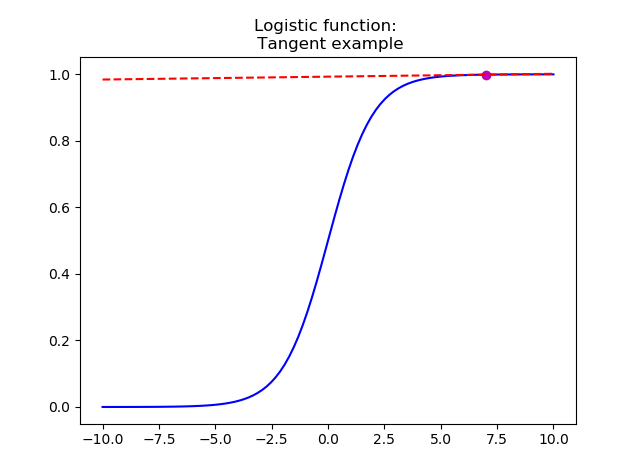
\includegraphics[scale = 0.7]{Figure2ANN.png}%
    \caption{\textbf{Example of a logistic function with a derivative evaluated at point x=7}}
    \label{fig4:ANN architecture}%
    \end{center}
\end{figure}

The number of layers and nodes are also hyperparameters. As for the learning rate or the batch size, there does not exist a universal method. Stathakis (2009) discuss the four different ways that are usually chosen to decide: Trial and error, heuristic search, exhaustive search (grid search), pruning and constructive algorithms. The most common way is to start with a rule of thumb and improving the model with trial and error. \par
The last element to choose is an activation function. For the last layer, the convention is to use a softmax or a logistic function for classification tasks. Now the remaining question is what activation function to use for the other layers. Glorot et al. (2011) advocate for the rectified linear unit (ReLU) where:

\begin{equation}\label{eq:17}
f(x) = max(0,x).
\end{equation}

Contrary to the step function see in the perceptron, ReLu is linear for $x>0$. The problem is that the hard 0 when $x<0$ can be complex to work with (as for the perceptron) but Glorot et al. proved that this property allows for sparsity which helps the network to train. There exist different approximation of ReLU like softplus where $f(x) = log(1+exp(x))$ or Leaky ReLU for which $f(x) = x $ if $x>0$ otherwise $f(x) = 0.01x$. 

\subsection{Ability to generalize}

We have seen in the last subsection how to optimize the network, but we never talked about generalization error. Many layers can be added and therefore include multiple nonlinear feature extraction. However, the deeper we go, the more the likelihood of the network to generalize well will be reduced.

The first way to avoid overfitting is to add a regularizer term to the error function such that we minimize :

\begin{equation}\label{eq:18}
\widetilde{E}(\boldsymbol{\omega}) = E(\boldsymbol{\omega}) + \frac{\lambda}{2}\boldsymbol{\omega}^T\boldsymbol{\omega}.
\end{equation}

Bishop(p.152-153) demonstrates that this regularizer is the same as adding a Gaussian prior distribution on the weights (since the error function is just the negative log likelihood). This regularizer term is governed by $\lambda$, a hyperparameter to choose in the network. When $\lambda=0$  the model is the original one. Adding this term, also called shrinkage parameter, will encourage the weights to converge to 0. When evaluating the derivative with respect to $\boldsymbol{\omega}$ the right term will be positive while we are trying to minimize the whole expression. A more general expression for this regularizer is 

\begin{equation}\label{eq:19}
\widetilde{E}(\boldsymbol{\omega}) = E(\boldsymbol{\omega}) + \frac{\lambda}{2}\|\boldsymbol{\omega}\|^q,
\end{equation}

which is the same as (5.22) when $q=2$. For example for the lasso regression $q=1$ which has some interesting properties for sparsity.

A second way to minimize the generalization error is early stopping. During the process of minimization of the objective function, the error is continuously decreasing (not necessarily the case for stochastic gradient descent). But after many iterations, the model starts to overfit, and the score on the out-of-sample data starts to deteriorate. Stopping the training before this iteration allows the model to generalize a lot better. 

The third and last way we shall present is dropout regularization. Introduced by Srivastava et al.(2014), dropout prevents overfitting by dropping out randomly some of the inputs meaning no calculation will be performed on the node. The randomness is obtained by using a Bernoulli distribution with probability $p$. In other words, each time an observation is passed through the network a node in the layer where we perform the dropout as probability $p$ to still be included in the feed-forward process. Dropout can be applied to each layer independently meaning different layers can have a different $p$. Figure 3, taken from the original paper, enables us to understand the architecture of the neural network resulting from the dropout process. Srivastava et al. compare this process to choosing a subsample of the network architecture randomly. Backpropagation is still performed the same way but for iterations where, let us say, $x_1$ has been dropped, then the gradient of the error function with respect to the weight associated to $x_1$ will be 0. The intuition behind why it works is what Srivastava et al. call co-adaptation. If all the nodes are present during the whole training step, then some features can rely on other features to correct errors. Dropping some of the nodes allows for certain features to be independent and therefore having a real change in the weights that correspond to the actual impact of the node. This method adds another hyperparameter, $p$, which, as for others, does not have a fixed rule and has to be chosen with trial and error.    

\begin{figure}[htb]%
    \begin{center}
    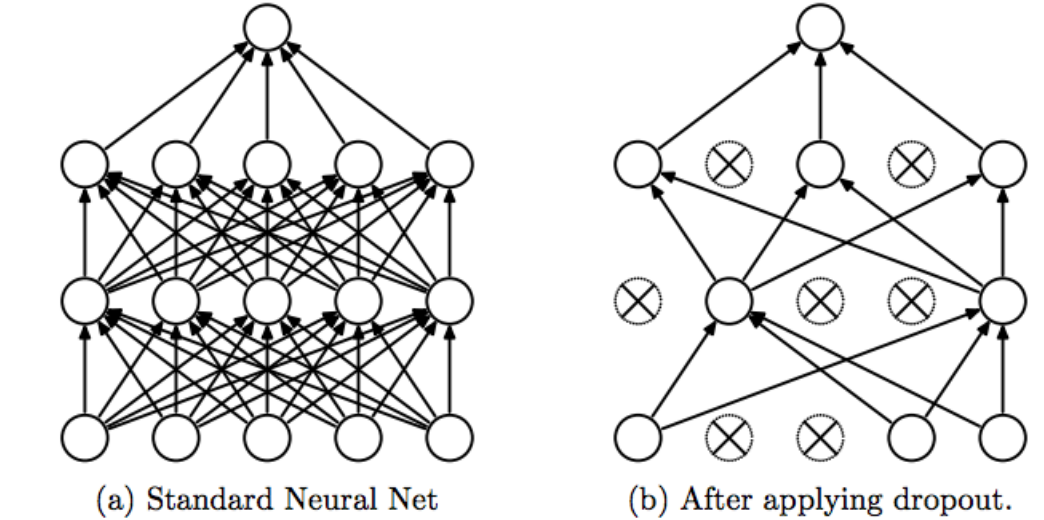
\includegraphics[scale = 0.5]{Figure3ANN.png}%
    \caption{\textbf{Example of dropout (Srivastava, 2014)}}
    \label{fig5:ANN dropout}%
    \end{center}
\end{figure}

In summary of this section. We have seen the underlying architecture of the deep neural network, how the forward propagation process works and then how the optimization algorithm, backpropagation, is performed. We then discussed briefly different arbitrary choice on parameters as in the learning rate or the type of activation function, and we ended with some solution to the recurrent problem of overfitting.

\newpage


\section{Additional algorithms}

This section will cover three more algorithms that we will use in the comparison: Logistic regression, k-nearest neighbor and naive Bayes. Since they are well known in the literature, we will not spend much time explaining them.

\subsection{Logistic regression}

Logistic regression uses the sigmoid function to predict the probability of a binary random variable $Y$, given $\boldsymbol{x}$ (observation) and $\boldsymbol{\beta}$ (parameters). $\beta$ is of dimension $(k x 1)$, and $\boldsymbol{x}$ $(1 x k)$.  The probability is then defined by :

\begin{align*}
Pr(Y = 1| \boldsymbol{x};\boldsymbol{\beta}) = \frac{1}{1+exp(-\boldsymbol{x}\boldsymbol{\beta})} \\
Pr(Y = 0| \boldsymbol{x};\boldsymbol{\beta}) = 1 - Pr(Y = 1| \boldsymbol{x};\boldsymbol{\beta}).
\end{align*}

The likelihood of a binary outcome variable for one observation is :

\begin{equation*}
Pr(Y = y| \boldsymbol{x};\boldsymbol{\beta}) = Pr(Y = 1| \boldsymbol{x};\boldsymbol{\beta})^yPr(Y = 0| \boldsymbol{x};\boldsymbol{\beta})^{1-y},
\end{equation*}

which is then generalized to $N$ observations and maximised. As in a neural network this sigmoid can be used in cases of a $K$ classes problem. The probabilities are then defined as :

\begin{align*}
Pr(Y = 1| \boldsymbol{x};\boldsymbol{\beta}) &= \frac{exp(\boldsymbol{x}\boldsymbol{\beta}_1)}{\sum_{k=1}^{K}exp(\boldsymbol{x}\boldsymbol{\beta}_k)} \\
                                             &\vdots \\
Pr(Y = K| \boldsymbol{x};\boldsymbol{\beta}) &= \frac{exp(\boldsymbol{x}\boldsymbol{\beta}_K)}{\sum_{k=1}^{K}exp(\boldsymbol{x}\boldsymbol{\beta}_k)} .
\end{align*}

In a more general way:

\begin{align*}
Pr(Y = c| \boldsymbol{x};\boldsymbol{\beta}) &= \frac{exp(\boldsymbol{x}\boldsymbol{\beta}_c)}{\sum_{k=1}^{K}exp(\boldsymbol{x}\boldsymbol{\beta}_k)} ,
\end{align*}

which is the softmax function. One of the parameter in $\boldsymbol{\beta}$ is then normalized so that the system is identifiable. Suppose the parameter substracted is the last, then $\boldsymbol{\beta}$ becomes $[\beta_1-\beta_K, \beta_2-\beta_K,..., \beta_{k-1}-\beta_K,0]$. In this case the likelihood becomes:

\begin{equation*}
Pr(Y = y| \boldsymbol{x};\boldsymbol{\beta}) = \Pi_{k=1}^{K} Pr(y=k|\boldsymbol{x};\boldsymbol{\beta})^{\mathbbm{1}[y = k]}
\end{equation*}

Which is once more generalized to N observations and maximized. In both cases, gradient-based methods can be used to optimize the respective likelihood with respect to $\boldsymbol{\beta}$.

\subsection{K-nearest neighbor}

Following once more Hastie et al. (2008), the k-nearest neighbor is a non-parametric algorithm which predicts a variable $Y$ for a new observation by taking into account the $k$ closest points from the training set. The basic procedure uses Euclidian norm as a measure of distance. In cases where $Y$ is continuous (regression) the predicted value is the average of the $Y$ value of the k neighbor :

\begin{equation*}
\hat{Y}(x) = \frac{1}{k}\sum_{x_i \in N_k(x)}y_i,
\end{equation*} 

with $\hat{Y}$ the predicted value for the new observation $x$, $N_k$ the $k$ closest points to x and $x_i$ the $i^{th}$ training observation where $i = 1, ..., N$. In cases where $Y$ is discrete (classification), the prediction is the class with the highest frequency in the neighborhood.  

\subsection{Naive Bayes}

Naive Bayes is a classification algorithm inspired by Bayes probabilities. The exposition is based on Zhang (2004). Let us define an observation, represented by the features $\boldsymbol{x}$ where $\boldsymbol{x} = (x_1, x_2, .., x_p)$. We want to predict a random variable $Y$ given the attributes $\boldsymbol{x}$ Therefore we can write:

\begin{equation*}
Pr(Y = k|\boldsymbol{x}) =\frac{Pr(\boldsymbol{x}|Y = k)Pr(Y = k)}{Pr(\boldsymbol{x})},
\end{equation*} 

which is the Bayes formula : posterior = (likelihood*prior)/evidence. The likelihood is of interest since evidence is just used to achieve a probability density and the prior is defined by the frequency of the class in the training set in most cases. 

\begin{equation*}
Pr(\boldsymbol{x}|Y = k) = Pr(x_1, x_2,..., x_p|Y = k).
\end{equation*}

Assuming that all the features are independent, we can rewrite the previous equation as:

\begin{equation*}
Pr(\boldsymbol{x}|Y = k) = \Pi_{p=1}^PPr(x_p|k).
\end{equation*}

This is a strong assumption which is rarely satisfied, and therefore the prediction power suffers from it. But the main advantage of this method is that it scales well. Depending on the type of data the likelihood will change. Common practice is to assume the normality distribution of each $x_i$ and to use the Gaussian probability distribution alongside with the mean and standard deviation to calculate each $Pr(x_i|c)$.\par
This finishes the short section about additional algorithms. We shall now present the experimental setup.



\newpage


\section{Experimental setup}

This section will be divided into 4 subsections. First, we will provide information concerning the datasets and the preprocessing of the dataset. The second subsection concerns the choice of hyperparameter. In the third subsection, we will discuss statistical tests used in the benchmark. Lastly, we shall present different performance measure.

\subsection{Datasets}

We used 12 Datasets described by Table 1. Alzheimer and Cell segment are both in the R package "AppliedPredictiveModelling" created by Kuhn and Johnson (2013). The NBA dataset was found on "data.world". The rest of the datasets can be found in the UCI machine learning repository (Dheeru and Taniskidou, 2017). Every dataset has a discrete variable $y$ that we try to predict.  \par
First, we check for missing values and delete the whole observation. We convert categorical data into binary dummies, which is a questionable choice since there exist different methods. Lessmann et al.(2015) used the weight of evidence method to do the transformation (other papers did not mention this step).  Following the same idea as Lessman et al.(2015) had for the class imbalance problem, we did not perform a feature selection algorithm. Some algorithms (e.g., random forest) are robust towards the selection of features. Therefore this gives us an idea of the true merit of the classifier and not some preprocessing algorithm such as L2 boosting. 

\begin{table}[h]
\begin{center}
\caption{Datasets}
\begin{threeparttable}
\begin{tabular}{ |c|c|c|c|c|c| } 
 \hline
 Dataset & Observations & Features & Categorical & Continuous & Classes \\ 
 \hline
 Adult & 30161 & 14 & 8 & 6 & 2 \\
 Alzheimer & 333 & 131 & 2 & 129 & 2 \\
 Marketing & 45211 & 16 & 9 & 7 & 2 \\
 Breast cancer & 569 & 30 & 0 & 30 & 2 \\
 Cell segment & 2019 & 116 & 0 & 116 & 2 \\
 Contraceptive method & 1473 & 9 & 7 & 2 & 3 \\ 
 Australian credit Approval & 690 & 14 & 8 & 6 & 2 \\
 Germany Credit Data & 1000 & 20 & 13 & 7 & 2 \\
 Iris & 150 & 4 & 0 & 4 & 3 \\
 Sonar & 208 & 60 & 0 & 60 & 2 \\
 Wine &178 & 13 & 0 & 13 & 3\\
 NBA & 1340 & 19 & 0 & 19 & 2 \\
 
 \hline
\end{tabular}
\begin{tablenotes}
\small
\item Note: Presentation of each Dataset with the number of observations in the sample, the number of features for each observation, the composition of the features (how many categorical and numerical value) and in the last column the number of groups. 
\end{tablenotes}
\end{threeparttable}
\label{table:1}
\end{center}
\end{table}


\newpage
\subsection{Choosing hyperparameters}

The benchmark was performed using seven algorithms: Deep neural network (DNN), Linear $C$-SVM (C-SVM), Radial basis function C-SVM (RBF SVM), random forest (RF), logistic regression (LR), k-nearest neighbor (KNN) and Gaussian naive Bayes (GNB). Before discussing the choice of hyperparameters, we need to define k-fold cross-validation, a model validation technique. 

K-fold cross-validation is an alternative method to hold-out. It consists of partitioning the dataset in $k$ sub-sample of equal size. We train the algorithm on $k-1$ fold (training set) and leave the last fold (testing set) to test the accuracy of the trained algorithm on an out-of-sample fold. This process is repeated k times in such a way so that each fold was used as a testing set once. The accuracy is then averaged to have some sense of how the model would perform on a new observation and check if the model overfits or not. Using the cross-validation with a grid-search approach allows us to find the model with the hyperparameters giving the most accuracy without overfitting.

To find the hyperparameters of C-SVM and RBF SVM we use the mentioned approach with $C = [0.1,1,10,100]$ for both and $ \gamma = [1e-07, 1e-05, 0.01, 0.1, 1] $. To solve SVM optimization we used the default method in python library meaning stochastic gradient descent for linear SVM and sequential minimal optimization for kernel SVM. In cases of a multiclass problem we use the OVA approach

In the neural network case, we fixed some hyperparameters with a rule of thumb. The number of layer was set to two and the number of node for layer 1 and layer 2 was set to $\sqrt{(m+2)N} + 2\sqrt{N/(m+2)}$ and $m\sqrt{N/(m+2)}$ respectively, as suggested in Huang (2003). For both layers, we used a reLu activation function due to the sparsity and computation advantages (Glorot et al., 2011). We fixed the batch size to 32 for computation purpose (The batch size is directly related to the memory). The optimization methods used were the stochastic gradient descent aswell as the Adam optimization with the default parameters of the library Keras. In each layer, weights were initialized with a uniform distribution. We then performed the same technique as for SVM to decide the number of epochs and the dropout rate with epochs = [32,64] and dropout rate = [0,0.1,0.2,0.3,0.4] for each layer. For datasets other than Adult and Marketing (due to the computation time of both) we continued to tune them by trial and error. Table 1 in the appendix shows the final choice of hyperparameters for each dataset.

For random forest we followed the advice of Hastie et al. (2008) to select the number of features selected in each split $m = \sqrt{p}$ with p the total number of features. We grow each tree to the end and choose the number of trees in the forest to be 128. We used the Gini index as a measure of error. 

For the logistic regression, we use the limited memory BFGS optimization algorithm. For the k-nearest neighbor, we use the rule of thumb $ k=\sqrt(N) $. 

\newpage
\subsection{Performance measure}

Now that we have presented the hyperparameters required to run the different algorithms, we need to discuss a way to evaluate their performance. The straightforward measure is the accuracy also called percentage correctly classified (PCC). The PCC is the proportion of observations that are correctly classified, in other words, observations for which the predicted class is equivalent to the true class. The PCC might not be appropriate especially for class imbalance problem (Ling and Sheng, 2011) that is why other measures have been proposed, and we will use PCC but also the F1-score and Matthew's correlation coefficient for the benchmark. For the definition of the F1-score we will follow {\"O}zg{\"u}r et al. (2005) and for the rest we base ourselves on Powers (2011).  To understand the difference between the three let us start by defining the confusion matrix.

\begin{table}[h]
\begin{center}
\caption{Confusion matrix}
\begin{tabular}{l|l|c|c|c}
\multicolumn{2}{c}{}&\multicolumn{2}{c}{True class}&\\
\cline{3-4}
\multicolumn{2}{c|}{}&Positive&Negative&\\
\cline{2-4}
\multirow{2}{*}{Predicted class}& Positive &  True positive(TP) & False positive(FP)& \\
\cline{2-4}
& Negative & False negative(FN) & True negative(TN) &\\
\cline{2-4}
\end{tabular}
\label{table:2}
\end{center}
\end{table}

From Table 2, we can define the accuracy as the sum of the diagonal divided by the sum of all the elements so $PCC = (TP+TN)/(TP+TN+FP+FN)$. Let us take an example where there is more observations with an actual value of negative class than positive. We shall set N to a 1000 with 990  observation in the negative class and only 10 in the positive. Now we perform two different classification algorithms, A and B, and observe the results. If algorithm A classified everything in the negative class therefore achieving a PCC of 0,99 (Table 3). Algorithm B predicted falsely 3 positive sample and 47 negative which gives a PCC of 0.95 (Table 4). Hence, according to the PCC performance measure, algorithm A outperforms algorithm B.

\begin{table}[h]
\begin{center}
\caption{Confusion matrix algorithm A}
\begin{tabular}{l|l|c|c|c}
\multicolumn{2}{c}{}&\multicolumn{2}{c}{True class}&\\
\cline{3-4}
\multicolumn{2}{c|}{}&Positive&Negative&\\
\cline{2-4}
\multirow{2}{*}{Predicted class}& Positive & 0 & 0& \\
\cline{2-4}
& Negative & 10 & 990 &\\
\cline{2-4}
\end{tabular}
\label{table:2}
\end{center}
\end{table}

\begin{table}[h]
\begin{center}
\caption{Confusion matrix algorithm B}
\begin{tabular}{l|l|c|c|c}
\multicolumn{2}{c}{}&\multicolumn{2}{c}{True class}&\\
\cline{3-4}
\multicolumn{2}{c|}{}&Positive&Negative&\\
\cline{2-4}
\multirow{2}{*}{Predicted class}& Positive &  7 & 47& \\
\cline{2-4}
& Negative & 3 & 943 &\\
\cline{2-4}
\end{tabular}
\label{table:2}
\end{center}
\end{table}


In some problems, predicting correctly positive samples might be of higher importance. That is usually the case in medicine where we rather want to diagnoses a patient as being positive for the disease, even if he is not, than having a negative result when he has the disease. This is also true for fraud detection, we would prefer to examine a false positive case rather than letting a crime go unnoticed. This problem is called "accuracy paradox" in the literature. To overcome this drawback, other measures should be used.

Going back to the confusion matrix we can create different performance score with each element. Using true positives and false positives we can create the positive predictive value (PPV) (also called precision) defined as :

\begin{equation*}
Precision = \frac{TP}{TP + FP}.
\end{equation*} 


A large number of false positives can lead to a low PPV. We can also use the recall measure:

\begin{equation*}
Recall = \frac{TP}{TP + FN}.
\end{equation*} 

A popular metric regrouping both mentioned performance score is the $F_1$ score. Exact definition and extension to the multiple classes of the $F_1$ score can be found in the appendix. Even though this performance score takes into account more information than a simple accuracy, it does not use the whole information available. Powers analyses different measures and shows that the Matthews correlation coefficient has some interesting properties, like using all of the available information. This coefficient is given by:

\begin{equation*}
MCC = \frac{TP*TN-FP*FN}{\sqrt{(TP + FP)(TP + FN)(TN + FP)(TN+FN)}}
\end{equation*}

In the results section, we present the accuracy in a table but will also present the result of the tests performed on the different type of performance evaluation. Another well-known performance score is the area under the receiving operator curve (AUROC), but we will not use it since it requires a probabilistic output which is not the case for the type of SVM we are using.

\newpage
\subsection{Statistical test}

Two of the most prominent paper in the field of comparison between classifiers are Diettrich (1998) and Demsar(2006). Diettrich focuses on the comparison of two learning algorithms trained on a small dataset. After giving a taxonomy of statistical questions and presenting five statistical tests, he performs a simulation and an experiment on real-world data in order to study type I error and the power of tests. The result of his paper was that the 5x2 cross-validation is more powerful than others but that McNemar is close behind. He recommends these two algorithms depending on the computational cost of the algorithm since in cross-validation the data needs to be fitted ten times. In practice, we often have two algorithms and a single dataset hence the importance of the work of Diettrich. \par
However, in our case, we want to compare multiple algorithms on multiple datasets. That is why we will use the work of Demsar who recommends using non-parametrical tests. He discussed the possible violation of different assumption in cases of t-tests: commensurability, normality, the absence of outliers. When comparing two algorithms on multiple datasets, he advises us to use the Wilcoxon signed-ranks test and the Friedman test in cases where we have multiple algorithms and multiple datasets. We shall use both tests with the appropriate post-hoc procedure since our main goal is to compare algorithms with logistic regression.  \par
The Wilcoxon signed-rank test is based on the paired difference of the two classifiers performance on each dataset. Since it is a paired difference it is an alternative to the paired t-test mentioned in Diettrich (1998) but without the normality constraint since it is a non-parametrical test. The first step of the test is to calculate the performance score of both algorithms on $N$ datasets giving us $Nx2$ performance score. Each score is then substracted pairwise resulting in N difference. Let us call $d_i$ the difference between performance scores of algorithm two and one on dataset $i$. Each absolute value of $d_i$ is then ranked by ascending order. Assume we have 2 datasets $(N=2)$ with $d_1 = 0$ and $d_2 = 0.03$. We give $d_1$ the rank 1 and $d_2$ the rank 2. If $d_1=d_2$ we will assign the rank 1.5 to both. The rank is assigned independently from the sign. Therefore in both case presented previously, if $d_2 = -0.03$ and $d_1=-d_2$  the rank would have stayed the same. Following Demsar notation, $R^+$ is the sum of the rank assigned to each $d_i \geq 0$ (The performance score of algorithm 2 was higher the one of algorithm 1) and $R^-$ the sum of rank assigned to $d_i \leq 0$

\begin{align*}
R^+ = \sum_{d_i>0}rank(d_i)+ \frac{1}{2}\sum_{d_i=0}rank(d_i) \\
R^- = \sum_{d_i<0}rank(d_i)+ \frac{1}{2}\sum_{d_i=0}rank(d_i)
\end{align*}

The statistic is then defined by $T= max(R^+,R^-)$. Since we have a small number of datasets, we must look on a table the exact critical value. For $\alpha = 0.05$, the null-hypothesis that the two algorithms give different performance score is rejected for $T$ below the critical value. 

The Friedman test ranks the performance score of each algorithm on a specific dataset. If algorithm one has a better score than algorithm two on dataset one, then their rank will respectively be 1 and 2 for this dataset. We repeat this operation $N$ times with $N$ the number of datasets. If there is a tie, an average rank is computed as in the Wilcoxon signed-rank test. The mean of the rank is then calculated for each algorithm. We explicitly give the rank in Table 5. Let us denote $r_i^j$ the rank of algorithm $j$ on dataset $i$ (with $j$ = 1, ..., $K$ and $i$ = 1, ..., $N$) and $R_j = \frac{1}{N}\sum_{i=1}^Nr_i^j$ the average rank of algorithm $j$. The statistic, taken from Friedman (1937), is:


\begin{equation*}
\chi^2 = \frac{K-1}{K\sigma^2}(\sum_{j=1}^KR_{j}-\rho)^2,
\end{equation*}

where $\rho$ and $\sigma^2$ are the mean and variance of $R_j$. The mean of the ranks is $ \rho = (1/2) (K+1)$ and the variance $\sigma^2 = (K^2-1)/(12N)$. We can rewrite the statistics as in Demsar:

\begin{equation*}
\chi^2 = \frac{12N}{K(K+1)}[\sum_{j=1}^KR^2_j-\frac{K(K+1)^2}{4}],
\end{equation*}

which follows a $\chi^2(K-1)$ distribution in case where $K$ and $N$ are big enough (Demsar gives the rule of thumb of $N$ > 10 and $K$ > 5). Demsar also present the Iman and Davenport correction:

\begin{equation*}
F = \frac{(N-1)\chi^2_F}{N(K-1)-\chi^2_F}. 
\end{equation*}

This new statistics follows a Fisher distribution F(K-1,(K-1)(N-1)) and is called Conover's F. The null hypothesis for this test is the equality of all average ranks, and the alternative is that at least one pair of average ranks are different. If the p-value of this test is less than 0.05 than the null hypothesis is rejected for a type one error fixed at 5\%. In cases where we reject H0, we need to perform a post-hoc analysis for pairwise comparison to see which algorithms are significantly different. There exist a plethora of such post-hoc tests. We will use the Nemenyi and Conover tests, provided by the "PMCMR" package in R. In both procedure Algorithm i is different from algorithm j if the difference $\|R_i-R_j\|$ is higher than a scalar. For Nemenyi this scalar is:

\begin{equation*}
\frac{q_{\infty;K;\alpha}}{\sqrt{2}}\sqrt{\frac{K(K+1)}{6N}}
\end{equation*}

With q the studenzied range distribution. The scalar for Conover is:

\begin{equation*}
t_{(\frac{1-\alpha}{2},(N-1)(K-1))}\sqrt{\frac{2K(1-\frac{\chi^2_R}{N(K-1)})(\sum_{i=1}^{N}\sum_{k=1}^KR^2_{i,j}-\frac{NK(k+1)^2}{4})}{(K-1)(N-1)}}
\end{equation*}

This finishes this section on the experimental setup. The last step is to perform the comparison. 




\newpage
\section{Results}

We have used 10-fold cross-validation and averaged them to get the different performance score. We reported the accuracy results in Table 5 along with their ranks necessary to perform the Friedman test. Interested readers can find the reports of F1 score and Matthew's correlation coefficient in the appendix.  

\begin{table}[h]
\begin{center}
\caption{Summary of accuracy}
\begin{threeparttable}
\begin{tabular}{ |c|c|c|c|c|c|c|c| } 
 \hline
 Dataset & LR & C-SVM RBF & C-SVM & RF & DNN & KNN & GNB \\ 
 \hline 
 Adult & 0.791 (3) & 0.795 (2) & 0.627 (7)& 0.850 (1) & 0.751 (6) & 0.771(5) & 0.789 (4)\\[1pt]
 Alzheimer & 0.841 (1) & 0.742 (4) & 0.730 (5) & 0.799 (2) & 0.787 (3)& 0.724 (6)& 0.687 (7) \\[1pt]
 Marketing & 0.891 (2) & 0.890(3) & 0.834 (7) & 0.906(1) & 0.884 (5) & 0.887 (4)& 0.852 (6)\\[1pt]
 Breast Cancer & 0.946 (2)& 0.923 (6) & 0.919 (7) & 0.965 (1) & 0.942 (3.5) & 0.930 (5) & 0.942 (3.5)\\[1pt]
 Cell segment & 0.750 (4) & 0.644 (7) & 0.678 (6) & 0.825 (1) & 0.683 (5)& 0.772 (2)& 0.758 (3) \\[1pt]
 Contraceptive & 0.508 (5) & 0.548 (2) & 0.506 (6) & 0.512 (4) & 0.557 (1) & 0.542 (3) & 0.445 (7) \\[1pt]
 Credit Aus & 0.852 (2) & 0.678 (7) & 0.788 (4) & 0.868 (1) & 0.795 (3) & 0.684 (6) & 0.785 (5) \\[1pt]
 Credit Ger & 0.728 (2) & 0.706 (4) & 0.572 (7) & 0.758 (1) & 0.700 (6) & 0.704 (5) & 0.707 (3)\\[1pt]
 Iris & 0.960 (4) & 0.967 (1.5) & 0.960 (4) & 0.947 (7) & 0.967 (1.5) & 0.960 (4) & 0.953 (6) \\[1pt]
 Sonar & 0.741 (4) & 0.865 (1) & 0.740 (5) & 0.816 (2) & 0.759 (3) & 0.654 (7) & 0.668 (6) \\[1pt]
 Wine & 0.955 (3) & 0.657 (7) & 0.854 (5) & 0.983 (1) & 0.916 (4) & 0.697 (6) & 0.978 (2) \\[1pt]
 NBA  & 0.703 (1.5) & 0.703 (1.5) & 0.601 (7) & 0.695 (3) & 0.694 (4) & 0.691 (5) & 0.624 (6) \\[1pt]
 \hline
 Average Ranks & 2.667  & 3.833 & 5.667 & 2.083 & 3.75 & 4.833 & 4.875 \\
 \hline

\end{tabular}
\begin{tablenotes}
\small
\item   Note: Accuracy of each algorithm on each dataset with their rank on the right parentheses.
\end{tablenotes}
\end{threeparttable}
\label{table:5}
\end{center}
\end{table}

Looking at table 5 the random forest seems to have the best accuracy score overall followed closely by logistic regression and neural networks. The average rank alone does not help us to conclude. We need to perform the appropriate statistical test. The Friedman rank test using the accuracy performance measure gives us the $\chi^2_F = 26,10226$, with a p-value of about 0.0002 meaning we can reject the null hypotheses that all average rank are similar. Conover's F is then equal to 6.256 and has a p-value of 3.056e-0.5 which confirms the above conclusion. The same decision can be observed for the F1-score and the Matthews correlation coefficient with a $\chi^2_F$ equal to 18.5 and 18.45 respectively. The next step is to perform a pairwise post-hoc test.  

\begin{table}[H]
\begin{center}
\caption{Nemenyi's post-hoc}
\begin{threeparttable}
\begin{tabular}{ |c|c|c|c|c|c|c|c| } 
 \hline
  & LR & C-SVM RBF & C-SVM & RF & DNN & KNN  \\ 
 \hline 
 C-SVM RBF & 0.90 & & & & & \\[1pt]
 C-SVM  & 0.0101 & 0.26 & & & &  \\[1pt]
 RF & 0.98 & 0.43 & 0.0004& & & \\[1pt]
 DNN & 0.93 & 1 & 0.22 & 0.49 & & \\[1pt]
 KNN & 0.2365 & 0.92 & 0.92 & 0.0301 & 0.88 & \\[1pt]
 GNB & 0.214 & 0.91 & 0.93 & 0.026 & 0.86 & 1 \\[1pt]
 \hline

\end{tabular}
\begin{tablenotes}
\small
\item   Note: each cell represents the p-value for the pairwise comparison between average ranks of the algorithm in column and row. the matrix being symetric we only fill the lower triangle. 
\end{tablenotes}
\end{threeparttable}
\label{table:6}
\end{center}
\end{table}

\begin{table}[H]
\begin{center}
\caption{Conover's post-hoc}
\begin{threeparttable}
\begin{tabular}{ |c|c|c|c|c|c|c|c| } 
 \hline
  & LR & C-SVM RBF & C-SVM & RF & DNN & KNN  \\ 
 \hline 
 C-SVM RBF & 0.91 & & & & & \\[1pt]
 C-SVM  & 0.013 & 0.28 & & & &  \\[1pt]
 RF & 0.99 & 0.45 & 0.0006 & & & \\[1pt]
 DNN & 0.94 & 1 & 0.24 & 0.51 & & \\[1pt]
 KNN & 0.26 & 0.93 & 0.93 & 0.036 & 0.89 & \\[1pt]
 GNB & 0.24 & 0.91 & 0.94 & 0.032 & 0.87 & 1 \\[1pt]
 \hline

\end{tabular}
\begin{tablenotes}
\small
\item   Note: each cell represents the p-value for the pairwise comparison between average ranks of the algorithm in column and row. 
\end{tablenotes}
\end{threeparttable}
\label{table:7}
\end{center}
\end{table}

Both post-hoc give the same results. At the value of $\alpha = 0.05$ only the random forest is different from C-SVM, KNN and naive bayes. The difference between logistic regression and C-SVM is only significant for $\alpha = 0.15$. For the post-hoc tests on the Matthews correlation coefficient and F1 score, only the difference between C-SVM and RF is different. The statistical tests show us that complex classifiers do not perform significantly better than usual ones like logistic regression. The Wilcoxon signed rank test also validates the absence of difference between logistic regression and C-SVM, RBF, RF and DNN.\par

This confirms the idea of Klambauer et al. (2017) who argues that the extensions of neural network such as convolutional neural network or recurrent neural network obtain the best performance in tasks such as image detection or natural language processing, but the classical feed-forward neural network rarely performs better than support vector machine or random forest (and in our case logistic regression).

On the other hand, the low significativity can be explained by multiple reasons. We only had twelve datasets which can be too small to detect any difference. Neural networks might also perform better than logistic regression in specific problems such as credit scoring, but in a general setting, with datasets fundamentally different, no significant results seem to emerge. Most of the hyperparameters in our network were set first by a rule of thumb and then updated by trial and errors, but we might not have found the optimal solution and accuracy could be improved in most cases. We never went deeper than two layers (even though the main features in the deep neural network is the number of layers, Klambhauer et al. (2017) mention that networks with many layers rarely succeed).

In summary, we found no evidence of a difference in performance score between logistic regression, support vector machine with a radial basis function kernel, random forest, and artificial neural network. This result should be taken with caution since our experimental setup can be flawed. However, we recommend scholars to use models like logistic regression, random forest or support vector machine as a starting point and only use the deep neural network when none of the above give satisfying results. Avoiding the complexity of neural networks while having decent results is a much-appreciated feature.   



\newpage
\section{Conclusion}

We present different machine learning algorithms and compare their performance with less complex algorithms, like the logistic regression, in the same way as Lessmann et al. (2015) did for the specific case of credit scoring. Our analysis was performed in a general setting with the help of non-parametrical statistical tests to overcome the flaws of the commonly used paired t-test and ANOVA. The experiment was conducted on twelve datasets with a classification problem. After a discussion on the different choices of hyperparameters and performance measure, we trained seven algorithms on each dataset and reported the score using the average of 10-fold cross-validation. We employed the Friedman test and Wilcoxon test recommended by Demsar as well as the appropriate post-hoc procedures (Nemenyi and Conover). We found that logistic regression, neural networks, random forests and support vector machines with a radial basis function as a kernel, performed equally well on three different performance score (Accuracy, F1-score, Matthews correlation coefficient). \par
We can avoid the complexity of a neural network and still have decent performance score. This conclusion is in accordance with Klambauher et al. (2017) but also with Cheng et al. (2018) who compared feed-forward neural network with polynomial regression and found no significant difference in performance. The experiment we made has its limitations. We had a low number of datasets, and the tuning of the neural network might not have been optimal. The deep neural network is a popular method but not well understood. \par
The next question that needs to be asked is about the differences in mathematical properties between algorithms like logistic regression and neural networks. Another interesting subject is the relation between recurrent neural network models (such as LSTM) and vector error correction model, both having the concept of short and long-term memory. This paper was only an introduction to the comparison between the neural network and other methods. Because deep learning methods are still considered as a black box, we foresee that more and more papers will try to explain the internal workings of the box. Comparison with other algorithms is one way to achieve this result, but it is not the only method.

\newpage

\singlespacing

\nocite{*}

\bibliographystyle{amsplain}
\bibliography{RevueV3}

\newpage
\begin{appendices}

\section{Performance measures}

\begin{equation*}
F_1 = 2\frac{Precision*Recall}{Precision + Recall} = 2\frac{TP}{2TP+FP+FN}
\end{equation*} 

In the case of a multi-class problem there is two way to calculate the $F_1$ score : Micro-average and macro-average. For micro-averaging we first redefine the precision and recall as:

\begin{equation*}
\overline{Precision} = \frac{\sum_{i=1}^K TP_i}{\sum_{i=1}^K(TP_i+FP_i)}
\end{equation*} 

\begin{equation*}
\overline{recall} = \frac{\sum_{i=1}^KTP_i}{\sum{i=1}^K(TP_i + FN_i)}
\end{equation*}

With $K$ the number of classes and $TP_i$ the true positive value for class i. The $F_1$ score is still the same formula but with $\overline{Precision}$  and $\overline{recall}$. For macro-average we compute the $F_1$ score for each  class ($F_i = (2*Precision_i*Recall_i)/(Precision_i + Recall_i)$)  and then calculate the mean:

\begin{equation*}
F_{macro}= \frac{1}{K}\sum_{i=1}^K F_i
\end{equation*}

The concept of macro and micro-average can also be used for the Matthews correlation coefficient.

\newpage
\section{Parameters of the deep neural network}


\begin{table}[H]
\begin{center}
\caption{Summary DNN parameters}
\begin{threeparttable}
\begin{tabular}{ |c|c|c|c|c|c|c|c| } 
 \hline
 Datasets & Batch size & Epochs & Optimization & \# of layer & \# of neurons & Dropout rates \\\hline 
\hline 
 Adult & 128 & 64 & Adam & 2 & (520, 173) &(0.5, 0.5)  \\[1pt]
 Alzheimer & 4 & 200 & Adam & 2 & (54,18)  & (0, 0) \\[1pt]
 Marketing & 32 & 64 & SGD & 2 & (637,212) & (0.3, 0.2)  \\[1pt] 
 Breast Cancer & 4 & 200 & Adam & 2 & (70,23) & (0.4, 0.2)\\[1pt]
 Cell segment & 32 & 128 & SGD & 2 & (133, 44) & (0, 0) \\[1pt]
 Contraceptive & 32 & 64 & Adam & 2 & (119, 51) & (0.2, 0.3)   \\[1pt]
 Credit Aus & 32 & 32 & Adam & 2 & (78,26) & (0.3, 0.4)  \\[1pt]
 Credit Ger & 30 & 32 & Adam & 2 & (94, 31) & (0.3, 0.4)\\[1pt]
 Iris & 4 & 200 & Adam & 1 & 37 & 0 \\[1pt]
 Sonar & 4 & 64 & Adam & 2 & (42, 14) & (0.2, 0.2)  \\[1pt]
 Wine & 4 & 200& Adam &  2 & (40, 17) & (0, 0)\\[1pt]
 NBA & 30 & 32 & Adam & 2 & (113, 48) & (0.1, 0.1)  \\[1pt]
 \hline



 \hline
\end{tabular}
\begin{tablenotes}
\small
\item   Note: The number of neurons and the dropout rates are assigned by layer so that the number on the left in parentheses is assigned to layer 1. 
\end{tablenotes}
\end{threeparttable}
\label{table: 8}
\end{center}
\end{table}



\section{Statistical tests on other performance measure}


\begin{table}[H]
\begin{center}
\caption{Summary of F1 scores}
\begin{threeparttable}
\begin{tabular}{ |c|c|c|c|c|c|c|c| } 
 \hline
 Dataset & LR & C-SVM RBF & C-SVM & RF & DNN & KNN & GNB \\ 
 \hline 
 Adult & 0.631 (3) & 0.626 (4) & 0.457 (6)& 0.789 (1) & 0.429 (7) & 0.510(5) & 0.646 (2)\\[1pt]
 Alzheimer & 0.782 (1) & 0.608 (6) & 0.627 (5) & 0.695 (3) & 0.703 (2)& 0.433 (7)& 0.651 (4) \\[1pt]
 Marketing & 0.629 (4) & 0.641(3) & 0.620 (5) & 0.724(1) & 0.503 (7) & 0.571 (6)& 0.688 (2)\\[1pt]
 Breast Cancer & 0.941 (2)& 0.914 (6) & 0.912 (7) & 0.962 (1) & 0.937 (3) & 0.921 (5) & 0.936 (4)\\[1pt]
 Cell segment & 0.711 (4) & 0.392 (7) & 0.571 (6) & 0.807 (1) & 0.598 (5)& 0.750 (2)& 0.746 (3) \\[1pt]
 Contraceptive & 0.481 (5) & 0.486 (3) & 0.468 (6) & 0.482 (4) & 0.528 (1) & 0.512 (2) & 0.441 (7) \\[1pt]
 Credit Aus & 0.850 (2) & 0.649 (7) & 0.780 (4) & 0.865 (1) & 0.790 (3) & 0.667 (6) & 0.772 (5) \\[1pt]
 Credit Ger & 0.651 (2) & 0.466 (5) & 0.397 (7) & 0.647 (3) & 0.411 (6) & 0.480 (4) & 0.664 (1)\\[1pt]
 Iris & 0.957 (4) & 0.961 (2) & 0.958 (3) & 0.941 (7) & 0.964 (1) & 0.951 (5) & 0.949 (6) \\[1pt]
 Sonar & 0.733 (4.5) & 0.861 (1) & 0.733 (4.5) & 0.807 (2) & 0.747 (3) & 0.635 (7) & 0.660 (6) \\[1pt]
 Wine & 0.951 (3) & 0.617 (7) & 0.834 (5) & 0.983 (1) & 0.903 (4) & 0.669 (6) & 0.978 (2) \\[1pt]
 NBA  & 0.670 (1) & 0.661 (5) & 0.559 (7) & 0.664 (3.5) & 0.665 (2) & 0.664 (3.5) & 0.623 (6) \\[1pt]
 \hline
 Average Ranks & 2.958  & 4.667 & 5.458 & 2.375 & 3.667 & 4.875 & 3.75 \\
 \hline

\end{tabular}
\begin{tablenotes}
\small
\item   Note: F1 macro-average score of each algorithm on each dataset with their rank on the right parentheses.
\end{tablenotes}
\end{threeparttable}
\label{table:9}
\end{center}
\end{table}

\begin{table}[H]
\begin{center}
\caption{Summary of Matthews correlation coefficient}
\begin{threeparttable}
\begin{tabular}{ |c|c|c|c|c|c|c|c| } 
 \hline
 Dataset & LR & C-SVM RBF & C-SVM & RF & DNN & KNN & GNB \\ 
 \hline 
 Adult & 0.348 (3) & 0.357 (2) & 0.201 (6)& 0.582 (1) & 0 (7) & 0.248(5) & 0.346 (4)\\[1pt]
 Alzheimer & 0.588 (1) & 0.281 (6) & 0.401 (4) & 0.456 (2) & 0.451 (7)& 0.017 (6)& 0.378 (5) \\[1pt]
 Marketing & 0.313 (4) & 0.325(3) & 0.307 (5) & 0.468(1) & 0.117 (7) & 0.232 (6)& 0.385 (2)\\[1pt]
 Breast Cancer & 0.884 (2)& 0.832 (7) & 0.835 (6) & 0.925 (1) & 0.876 (3.5) & 0.848 (5) & 0.876 (3.5)\\[1pt]
 Cell segment & 0.437 (4) & 0 (7) & 0.279 (6) & 0.617 (1) & 0.298 (5)& 0.503 (3)& 0.504 (2) \\[1pt]
 Contraceptive & 0.228 (5) & 0.287 (3) & 0.219 (6) & 0.236 (4) & 0.315 (1) & 0.289 (2) & 0.197 (7) \\[1pt]
 Credit scr Aus & 0.705 (2) & 0.348 (7) & 0.583 (4) & 0.734 (1) & 0.586 (3) & 0.356 (6) & 0.567 (5) \\[1pt]
 Credit scr Ger & 0.316 (3) & 0.127 (4) & 0.064 (6) & 0.357 (1) & 0 (7) & 0.114 (5) & 0.337 (2)\\[1pt]
 Iris & 0.942 (3.5) & 0.951 (2) & 0.942 (3.5) & 0.922 (7) & 0.953 (1) & 0.940 (5) & 0.932 (6) \\[1pt]
 Sonar & 0.498 (4) & 0.726 (1) & 0.492 (5) & 0.641 (2) & 0.533 (3) & 0.319 (7) & 0.396 (6) \\[1pt]
 Wine & 0.931 (3) & 0.497 (7) & 0.792 (5) & 0.974 (1) & 0.874 (4) & 0.540 (6) & 0.967 (2) \\[1pt]
 NBA  & 0.351 (1) & 0.348 (2) & 0.274 (7) & 0.336 (4.5) & 0.338 (3) & 0.336 (4.5) & 0.323 (6) \\[1pt]
 \hline
 Average Ranks & 2.958  & 4.25 & 5.292 & 2.208 & 4.292 & 5.042 & 4.208 \\
 \hline

\end{tabular}
\begin{tablenotes}
\small
\item   Note: Matthews correlation coefficient micro-average score of each algorithm on each dataset with their rank on the right parentheses. 
\end{tablenotes}
\end{threeparttable}
\label{table:10}
\end{center}
\end{table}

\begin{table}[H]
\begin{center}
\caption{Nemenyi's post-hoc on F1score}
\begin{threeparttable}
\begin{tabular}{ |c|c|c|c|c|c|c|c| } 
 \hline
  & LR & C-SVM RBF & C-SVM & RF & DNN & KNN  \\ 
 \hline 
 C-SVM RBF & 0.456 & & & & & \\[1pt]
 C-SVM  & 0.069 & 0.973 & & & &  \\[1pt]
 RF & 0.995 & 0.126 & 0.0086& & & \\[1pt]
 DNN & 0.985 & 0.918 & 0.395 & 0.766 & & \\[1pt]
 KNN & 0.310 & 1 & 0.995 & 0.069 & 0.818 & \\[1pt]
 GNB & 0.902 & 0.989 & 0.647 & 0.519 & 1 & 0.956 \\[1pt]
 \hline

\end{tabular}
\begin{tablenotes}
\small
\item   Note: each cell represents the p-value for the pairwise comparison between average ranks of the algorithm in column and row.
\end{tablenotes}
\end{threeparttable}
\label{table:6}
\end{center}
\end{table}

\begin{table}[H]
\begin{center}
\caption{Nemenyi's post-hoc on Matthews correlation coefficient}
\begin{threeparttable}
\begin{tabular}{ |c|c|c|c|c|c|c|c| } 
 \hline
  & LR & C-SVM RBF & C-SVM & RF & DNN & KNN  \\ 
 \hline 
 C-SVM RBF & 0.818 & & & & & \\[1pt]
 C-SVM  & 0.141 & 0.902 & & & &  \\[1pt]
 RF & 0.965 & 0.237 & 0.009& & & \\[1pt]
 DNN & 0.945 & 1 & 0.738 & 0.425 & & \\[1pt]
 KNN & 0.215 & 0.956 & 1 & 0.016 & 0.842 & \\[1pt]
 GNB & 0.883 & 1 & 0.842 & 0.31 & 1 & 0.9178 \\[1pt]
 \hline

\end{tabular}
\begin{tablenotes}
\small
\item   Note: each cell represents the p-value for the pairwise comparison between average ranks of the algorithm in column and row.
\end{tablenotes}
\end{threeparttable}
\label{table:11}
\end{center}
\end{table}

\begin{table}[H]
\begin{center}
\caption{Conover's post-hoc on F1 score}
\begin{threeparttable}
\begin{tabular}{ |c|c|c|c|c|c|c|c| } 
 \hline
  & LR & C-SVM RBF & C-SVM & RF & DNN & KNN  \\ 
 \hline 
 C-SVM RBF & 0.486 & & & & & \\[1pt]
 C-SVM  & 0.082 & 0.976 & & & &  \\[1pt]
 RF & 0.995 & 0.146 & 0.011 & & & \\[1pt]
 DNN & 0.987 & 0.926 & 0.425 & 0.786 & & \\[1pt]
 KNN & 0.339 & 1 & 0.995 & 0.082 & 0.834 & \\[1pt]
 GNB & 0.911 & 0.990 & 0.673 & 0.548 & 1 & 0.961 \\[1pt]
 \hline

\end{tabular}
\begin{tablenotes}
\small
\item   Note: each cell represents the p-value for the pairwise comparison between average ranks of the algorithm in column and row.
\end{tablenotes}
\end{threeparttable}
\label{table:12}
\end{center}
\end{table}

\begin{table}[H]
\begin{center}
\caption{Conover's post-hoc on Matthews correlation coefficient}
\begin{threeparttable}
\begin{tabular}{ |c|c|c|c|c|c|c|c| } 
 \hline
  & LR & C-SVM RBF & C-SVM & RF & DNN & KNN  \\ 
 \hline 
 C-SVM RBF & 0.834 & & & & & \\[1pt]
 C-SVM  & 0.162 & 0.911 & & & &  \\[1pt]
 RF & 0.969 & 0.262 & 0.011 & & & \\[1pt]
 DNN & 0.951 & 1 & 0.758 & 0.454 & & \\[1pt]
 KNN & 0.240 & 0.961 & 1 & 0.021 & 0.856 & \\[1pt]
 GNB & 0.894 & 1 & 0.856 & 0.338 & 1 & 0.926 \\[1pt]
 \hline

\end{tabular}
\begin{tablenotes}
\small
\item Note: each cell represents the p-value for the pairwise comparison between average ranks of the algorithm in column and row.
\end{tablenotes}
\end{threeparttable}
\label{table:13}
\end{center}
\end{table}



\end{appendices}



\end{document}